\documentclass[%
 aip,
% jmp,
% bmf,
% sd,
% rsi,
 amsmath,amssymb,
%preprint,%
 reprint,%
%author-year,%
%author-numerical,%
% Conference Proceedings
]{revtex4-1}

\usepackage{graphicx}
\usepackage{dcolumn}
\usepackage{bm}
\usepackage{hyperref}
\usepackage[utf8]{inputenc}
\usepackage[T1]{fontenc}
\usepackage{mathptmx}
\usepackage{etoolbox}
\usepackage{subfigure}

\makeatletter
\def\@email#1#2{%
 \endgroup
 \patchcmd{\titleblock@produce}
  {\frontmatter@RRAPformat}
  {\frontmatter@RRAPformat{\produce@RRAP{*#1\href{mailto:#2}{#2}}}\frontmatter@RRAPformat}
  {}{}
}
\makeatother
\begin{document}

\preprint{AIP/123-QED}

\title[Single-photon emission from CdSe quantum dots]{Observation of single-photon emission with nanosecond lifetimes from colloidal cadmium selenide quantum dots}

\author{Manojkumar V, Geetha K. Varier, Radhika Vathsan, P. Nandakumar}
 \email{nandan@goa.bits-pilani.ac.in}
 
\affiliation{Department of Physics, Birla Institute of Technology \& Science, Pilani, K K Birla Goa Campus, Goa 403726, India}

\date{\today}

\begin{abstract}
High repetition rate single-photon emitters are essential for all-optical quantum information processing, communications and metrology. The spontaneous emission lifetimes of semiconductor quantum dots are typically of the order of 10 ns, severely limiting their brightness and therefore their potential applications in quantum devices.  Here, we report on single-photon emission with nanosecond lifetime from cadmium selenide quantum dots embedded in a polymer matrix. The study shows that the emission lifetime can be tuned by appropriately choosing the particle size and the dielectric constant of the surrounding medium. The quantum dots are synthesized using a green synthesis protocol and surface passivated using oleic acid. A Hanbury Brown and Twiss setup attached to an in-house constructed confocal microscope is used to efficiently couple and characterize the single-photon emission from an array of quantum dots.  Detailed analysis of the second-order correlation function ($g^{(2)}(\tau)$) of single-photon emission from cadmium selenide quantum dots reveals the particle size dependence of emission lifetimes. The study also shows that the quality of single-photon emission, as revealed by $g^{(2)}(0)$, reduces with increasing particle size in the strongly confined regime.
\end{abstract}

\maketitle

\section{\label{sec:level1}Introduction}
 Quantum dots (QDs) are nanometer-sized semiconductor crystallites typically consisting of tens to a few thousands of atoms or molecules,  forming an integral system. The physical \cite{CC, DD, EE} and chemical\cite{AA, BB} properties  of quantum dots undergo significant change due to the confinement of charge carriers within the material \cite{AAM}. The quantum confinement effect is pronounced when the size of the quantum dots is less than the de Broglie wavelength of the charge carriers. Quantum confinement results in remarkable changes in the density of states, leading to the formation of discrete energy levels rather than the continuous energy bands normally observed in bulk solids \cite{AAO}. Semiconductor QDs, with their discrete energy levels, are one of the potential candidate materials for developing single-photon sources for quantum technologies. On-demand single-photon sources are integral to any optical implementation of quantum technologies, crucial in quantum communication\cite{AAG} and quantum metrology \cite{AAH}, and are part of any quantum optics lab focusing on experiments on foundations of quantum physics \cite{AAI}.

The quest for developing on-demand single-photon sources with high brightness (high repetition rate of single photons) has gained much momentum in recent years. \cite{OO, XX}. A higher repetition rate of photons is normally achieved by increasing the spontaneous emission rate by coupling single-photon sources to plasmonic cavities \cite{PP}. However, this technique inherently leads to a higher probability of multiple photons emission \cite{QQ}.  Epitaxially grown cadmium selenide quantum dots (CdSe QDs) on zinc selenide have suppressed non-radiative phenomena at higher temperatures, thereby decreasing the radiative lifetime \cite{RR}. However, the molecular beam epitaxy system is a complicated and expensive technique. Here, we report on the nanosecond radiative lifetimes observed in colloidal CdSe QDs in a dielectric matrix, emitting single photons at room temperature. To our knowledge, single-photon emission from colloidal CdSe QDs at room temperature with size-dependent life times has not been reported so far.

Cadmium selenide is a group II-VI chalcogenide compound with a direct bulk bandgap of 1.74 eV, which can be increased by decreasing the crystal size. Each selenium anion is surrounded by four cadmium cations and vice versa to form a tetrahedral structure that resembles $sp^3$ hybridization. This indicates the presence of characteristics associated with both covalent and ionic bonding \cite{AAE}. Colloidal  synthesis of CdSe QDs is usually done by the conventional hot-injection method, which involves the rapid mixing of reagents at high temperatures \cite{NN}. However, the difficulty in introducing large amounts of reagents into the mother solution in a very short time creates an insurmountable drawback in this type of synthesis. In addition, the reaction temperature needs to decrease after the injection step to confine nucleation to a brief interval and slow down subsequent growth of nanocrystals. Since the cooling rate does not scale linearly with the reaction volume, the uniformity in the QD size is affected\cite{FF}. A two-fold change in the size of QDs typically results in a shift of tens of nanometers in emission wavelengths, which poses a severe limitation in applications where photon indistinguishability is crucial \cite{GG}. Some of these drawbacks can be overcome by using heat-up synthesis techniques. This  involves mixing two precursors at higher temperatures and promotes slow growth of nanocrystals, for better control over the size.

Colloidal CdSe QDs are associated with lattice defects that result in Auger recombination \cite{II}. This provides a pathway for non-radiative recombination by transferring the energy from electron-hole pair recombination to another electron (or hole) that is subsequently excited to the defect level \cite{UU}. This phenomenon is depicted with the presence of an intermediate energy level (IS) between the ground state (GS) and the excited state (ES),  in Figure \ref{fig: energy level diagram}. Due to the negligible time scale of transitions within the energy bands compared to the time scale of the radiative transition, the bands are approximated by discrete single-energy levels \cite{TT}. The higher probability of electronic transition mediated by the IS increases the quenching of emission \cite{UU} resulting in shorter lifetime \cite{AAJ} of the ES. Quenching can be reduced by passivating the surface states of each QD with surfactants. This reduces the likelihood of non-radiative recombination processes occurring due to the presence of surface defects or dangling bonds, that might trap charge carriers \cite{AAU}. Surfactants such as oleic acid contain a carboxylate chain and have an anionic nature \cite{AAF}; they attach to the excess cadmium cations on the surface to prevent the aggregation of QDs as well. 

\begin{figure}
    \centering
    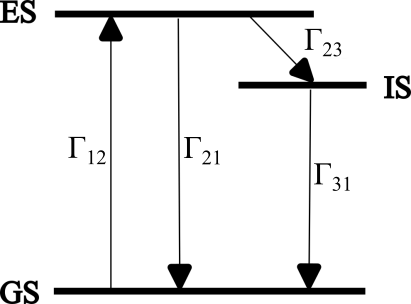
\includegraphics[width=0.55\linewidth]{energy level diagram.png}
    \caption{Energy-level diagram for a three-level system of colloidal CdSe QDs. An electron is excited from the ground state (GS) to an excited state(ES) with the transition rate \textbf{$\Gamma_{12}$} upon absorbing a photon of energy equivalent to $(ES-GS)$. This electron either transits  to  GS with the rate $\Gamma_{21}$ by emitting a photon or non-radiatively transits to an intermediate state (IS) with the rate $\Gamma_{23}$, due to the presence of defects and then transits from IS to GS with the rate $\Gamma_{31}$ by emitting a photon.}
    \label{fig: energy level diagram}
\end{figure}


The present work focuses on increasing the repetition rate of single-photon emission from colloidal QDs without using an external cavity. CdSe QDs studied so far have a radiative lifetime of the order of ten nanoseconds \cite{AAV}. In this work, an order of magnitude reduction in the radiative lifetime is achieved by (i)~making use of QDs in the intermediate confinement regime and (ii)~immersing QDs in a medium of higher dielectric constant. The lifetime of the excited states is determined by studying the single-photon emission from isolated quantum dots and analyzing the second-order correlation function. 
The lifetime study is conducted by exciting the QDs with a continuous wave (CW) laser, requiring no  high-power ultrafast laser. Experiments are carried out using a confocal microscope attached to a Hanbury Brown and Twiss (HBT) interferometer. An array of well-separated QDs in the form of a thin film is studied using the setup which allows for probing different QDs by moving the focal spot with ease. Further, we elucidate the correlation between the lifetime and size of the individual CdSe QDs by comparing the distribution of the lifetime of QDs in an array with their size distribution. Efficient coupling of an array of single-photon emitters at room temperature is of paramount importance in quantum technologies.

\section{\textbf{EXPERIMENTAL METHODS AND SETUP}}

\subsection{\textbf{Synthesis and sample preparation of colloidal CdSe QDs}}
Colloidal CdSe QDs are synthesized using a green synthesis method as follows \cite{AAK}. 1~ml of 5~mM selenium precursor is prepared by dissolving elemental selenium ($>$ 99.5~\% purity, Sigma Aldrich) in olive oil at 200$^\circ$C for 2 hours and subsequently cooling to room temperature. 5 ml of 10 mM cadmium precursor is prepared by dissolving cadmium oxide powder ($>$ 99~\% purity, Nice Chemicals) in olive oil at 300$^\circ$C for 30 minutes. 60~$\mu$l of oleic acid ($>$ 97~\% purity, Spectrochem) is added to the cadmium precursor while heating. Cooled selenium precursor is then immediately added to hot cadmium precursor, with a sudden lowering of temperature to 280$^\circ$C. This solution is heated for 1 hour at 300$^\circ$C. 
The hot solution is immediately poured into 40~ml acetone (Sigma Aldrich), forming a precipitate. This is centrifuged at 2000 rpm for 10 minutes to allow the precipitate to separate from the supernatant. The supernatant is decanted, and this process repeated four more times to remove the residual olive oil. The final precipitate is added to 2~ml toluene (99.9~\% purity, Sigma Aldrich) for characterization, without further purification.

The procedure to prepare a thin film of CdSe QDs for confocal microscope imaging is as follows: 

\noindent 50 mg of  polymethyl methacrylate (PMMA) powder (molecular weight 120,000, Sigma Aldrich) is added to 1~ml toluene. This is heated at 50$^\circ$C until a clear transparent solution is obtained. The polymer solution is added to 20~$\mu$l of concentrated CdSe QD solution to prepare a stock solution. This stock is diluted further in 1 ml toluene. This mixture is sonicated for 40 minutes. 20~$\mu$l of this mixture is spin-coated at 1000 rpm for 60 seconds on a coverslip to form a thin film of uniform thickness. The obtained transparent polymer film contains monodispersed QDs and is used for confocal microscope imaging. The dilution of CdSe QDs is chosen such that the spin-coated film has a particle density of less than 1 per $\mu$m$^{-2}$ area.


\subsection{\textbf{Confocal  Hanbury Brown and Twiss  microscope for characterization of single-photon emission}}
The spin-coated CdSe QDs film is imaged using a confocal microscope  that was constructed in-house\cite{HH}. A schematic diagram of the experimental setup is shown in Figure \ref{fig:experimental setup}. A continuous wave laser beam of wavelength 543~nm is used to excite the particles in the film. This beam is focused onto the film by a 60X oil immersion objective (NA = 1.25, UPlanFLN 60X, Olympus) attached to Olympus IX71 inverted microscope. ScanImage software (Vidrio Technologies) is used to communicate with the data acquisition card (NI-USB-6356) to control both the XY scanning galvo-mirror system (GVS002/M, Thorlabs) (not shown in the figure) and photomultiplier tube PMT (H7732-10, Hamamatsu Photonics). Fluorescence light emitted from the film is transmitted through a dichroic mirror (DM) (ZT488/543rpc, Chroma Technology Corp) and is allowed to fall on the photo-multiplier tube (PMT). A typical 2D image of CdSe QDs film as shown in Figure \ref{fig:single frame} is obtained by raster scanning  the sample using XY scanning galvo-mirrors system.

\begin{figure}
    \centering
    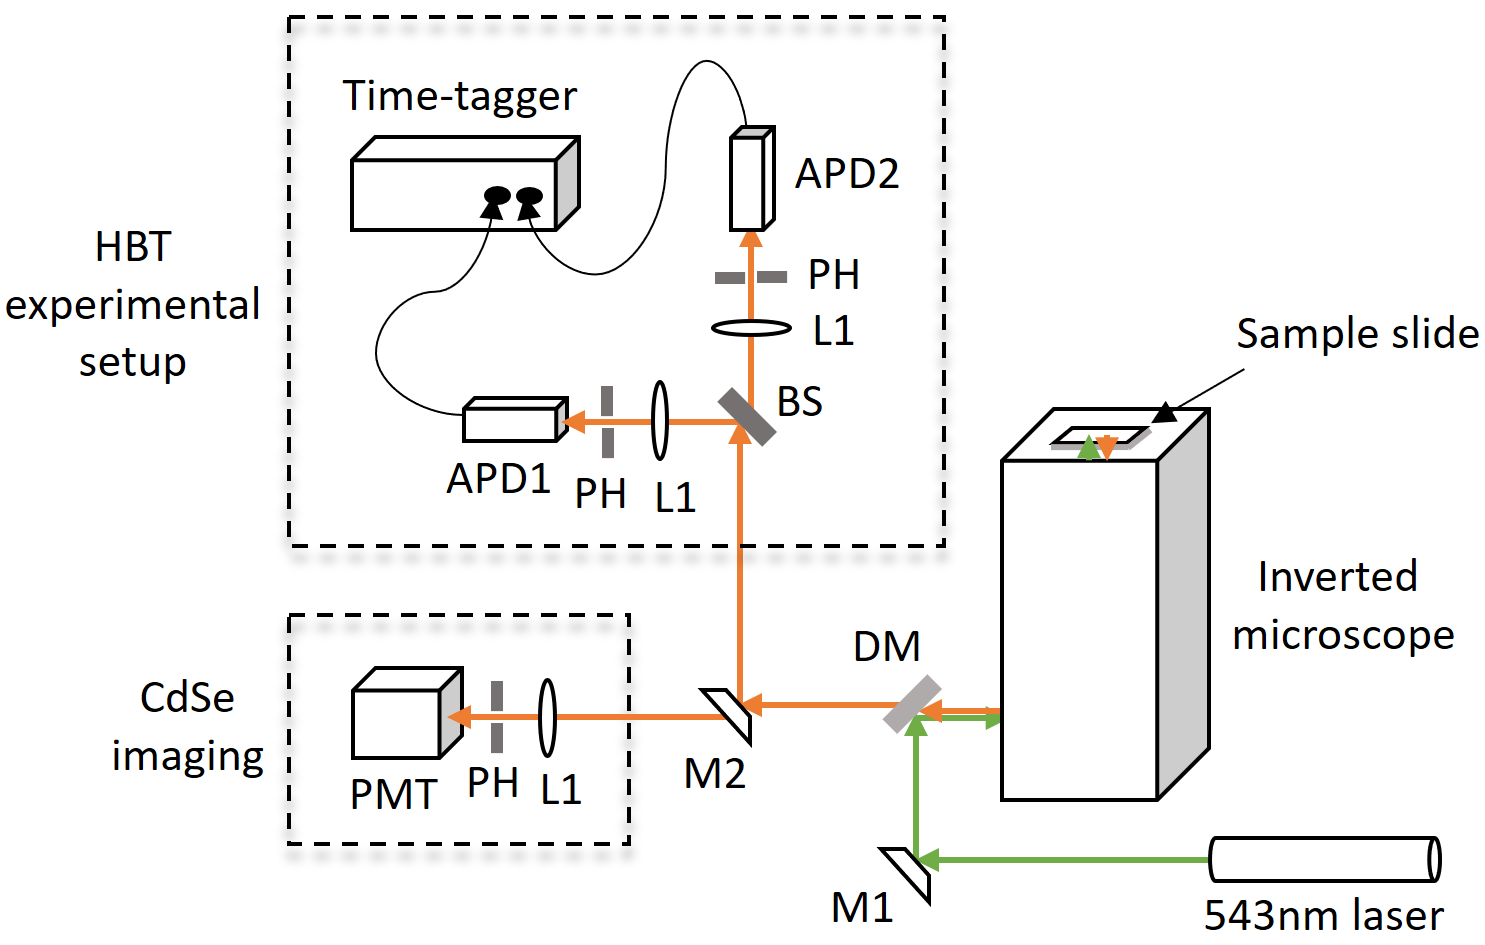
\includegraphics[width=1\linewidth]{experimental setup.png}
    \caption{Experimental setup for imaging and detection of single photon emitters. M1---fixed mirror,  M2---flip mirror; DM---dichroic mirror, BS---50\% beam splitter, L1---lens, PH---pinhole, APD---avalanche photodiode, PMT---photomultiplier tube.}
    \label{fig:experimental setup}
\end{figure}


Once the confocal image of CdSe QDs is obtained, a particular QD is selected and the laser beam is continuously focused onto it through the microscope objective. The fluorescence from this QD is then directed into the HBT setup with the help of the flip mirror M2. The HBT setup consists of a 50--50 beam splitter (BS) from which  two equal-intensity output beams are focussed onto the active area of avalanche photodiodes APD1 and APD2 (350~ps resolution, SPCM AQRH-14FC, Excelitas Technologies), through lenses L1 of 5~cm focal length.  Pinholes PH placed after L1 in each arm eliminate the light from the out-of-focal-plane reaching APDs. These APDs generate an output TTL pulse upon each photon-detection event,  the timings of which  are recorded using a time-tagger (81~ps resolution, ID800, ID Quantique). An algorithm written in Matlab constructs a histogram of the number of photons reaching the detectors with time delay $\tau = |t - t'|$, where $t$ and $t'$ are the recorded time of arrival of photons in APD1 and APD2 respectively. The quality of single-photon emission is studied by computing the normalized second-order correlation function $g^{(2)}(\tau)$. This relates the probability of detecting a photon at a time $t$ to the probability of detecting another photon at a later time $t'$ and is defined by
\begin{equation}
g^{(2)}(\tau) = \frac{\langle n_1(t) \rangle \langle n_2(t+\tau) \rangle}{\langle n_1(t) n_2(t+\tau) \rangle}
\end{equation}
\noindent where $\langle n_1 \rangle $ and $\langle n_2 \rangle$ are the  time-averaged count rates of photons in APD1 and APD2 respectively. For all practical single-photon sources, $g^{(2)}(0)$ is close to zero, the expected value for  an ideal single-photon source. 


\section{\textbf{RESULTS AND DISCUSSION}}

\subsection{\textbf{Imaging of CdSe QDs}}
The spin-coated film of monodispersed CdSe QDs in PMMA polymer matrix is imaged using the confocal microscope setup. A sample image of the QDs from an area of 16~$\mu$m$^2$ is shown in Figure \ref{fig:single frame}. The average diameter of the bright spots is 280~nm, which is the expected diffraction-limited spot size. The horizontal stripes seen on bright spots in the confocal image are due to the photoluminescence blinking \cite{II} resulting from Auger recombination.
\begin{figure}
    \centering
    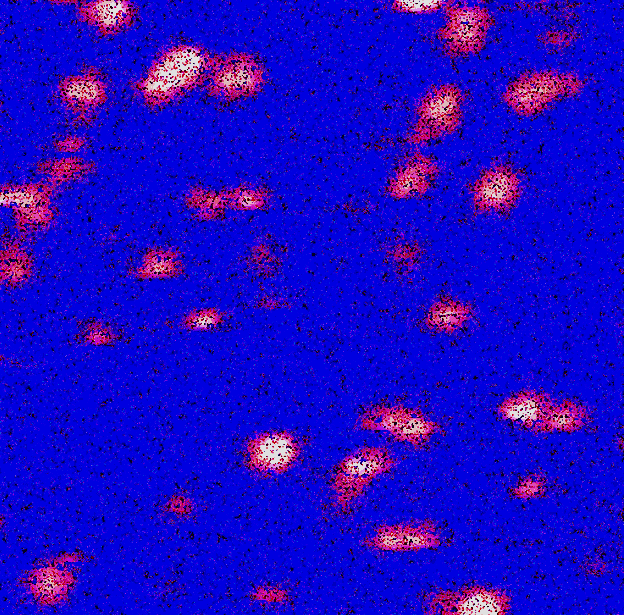
\includegraphics[width=0.7\linewidth]{single frame.jpg}
    \caption{Confocal microscope image of colloidal CdSe QDs of 16~$\mu$m$^2$ area. Each bright spot has a diameter of about 280~nm, implying diffraction-limited imaging.}
    \label{fig:single frame}
\end{figure}


\subsection{\textbf{Second-order correlation function}}
Single-photon emission from individual CdSe QDs is characterized using the HBT setup (Figure \ref{fig:experimental setup}). A typical plot of the second-order correlation function $g^2(\tau)$ is shown in Figure \ref{fig:g2 measurement}. Each black circle in the figure refers to the number of photon-pair detection events in APD1 and APD2 with a time delay $\tau = |t - t'|$. The second-order correlation function for a three-level system is related to the transition lifetimes by \cite{SS, TT}
\begin{equation}
g^{(2)}(\tau)=1-(1+b)e^{-\lambda_1 |\tau|}+be^{-\lambda_2 |\tau|},
\label{eq:gtwo}
\end{equation}
\noindent where $\lambda_1$ is the decay constant corresponding to ES$\leftrightarrow$GS transition.  $\lambda_1 \sim \Gamma_{12} + \Gamma_{21}$ where $\Gamma_{12}$ and $\Gamma_{21}$ are the rate constants corresponding to absorption and subsequent spontaneous emission from level ES to level GS, respectively (see Figure \ref{fig: energy level diagram}). However, for low power excitation, as is the case here, the decay constant $\lambda_1$ is dominated by the decay rate of the excited state, $\Gamma_{21}$ being an order magnitude higher than $\Gamma_{12}$ \cite{TT}. $\lambda_2$ is the transition rate mediated by the ES$\rightarrow$IS $\rightarrow$GS transition. The second term of eq.\eqref{eq:gtwo} reflects photon-antibunching and causes a dip to appear in the correlation function at $\tau = 0$. This behavior arises because the QD re-emits a photon only after the excited state has decayed by emitting the first photon. The third term in the above equation is responsible for the blinking of emission, which arises due to the inherent defect states of colloidal CdSe QDs \cite{KK}. The coefficients corresponding to the second and third terms represent the amplitude of transitions to ES and IS respectively.
 
The correlation data ($\circ$) in Figure (\ref{fig:g2 measurement}) is fitted to the behavior predicted by eq. (\ref{eq:gtwo}) for a three-level system after deconvolution (red curve) with the instrument response function of 360 ps. This fit gives the parameters $b$, $\lambda_1$ and $\lambda_2$ of eq. (\ref{eq:gtwo}). The lifetime $t_1 = 1/\Gamma_{21}$  of the excited state, is approximately equal to $1/\lambda_1$, as discussed earlier. The value of $g^{(2)}(0)$ in this figure is close to zero.  The non-zero value of $g^{(2)}(0)$ could arise due to various reasons, such as (i) weak multiple photons generated from the biexciton cascade \cite{WW}, (ii) a fraction of scattered laser light reaching the detectors that increase with the incident power. The noise around $\tau = 0$ in $g^{(2)}(\tau)$ plot could arise from (i) the photons emitted at random times due to the slow decay component $t_2$ \cite{XX}, (ii) from the shot noise associated with the laser and APDs. The appearance of wings around the dip is associated with the third term of eq. (\ref{eq:gtwo}) that signifies the exhibition of photoluminescence blinking.

\begin{figure}
    \centering
    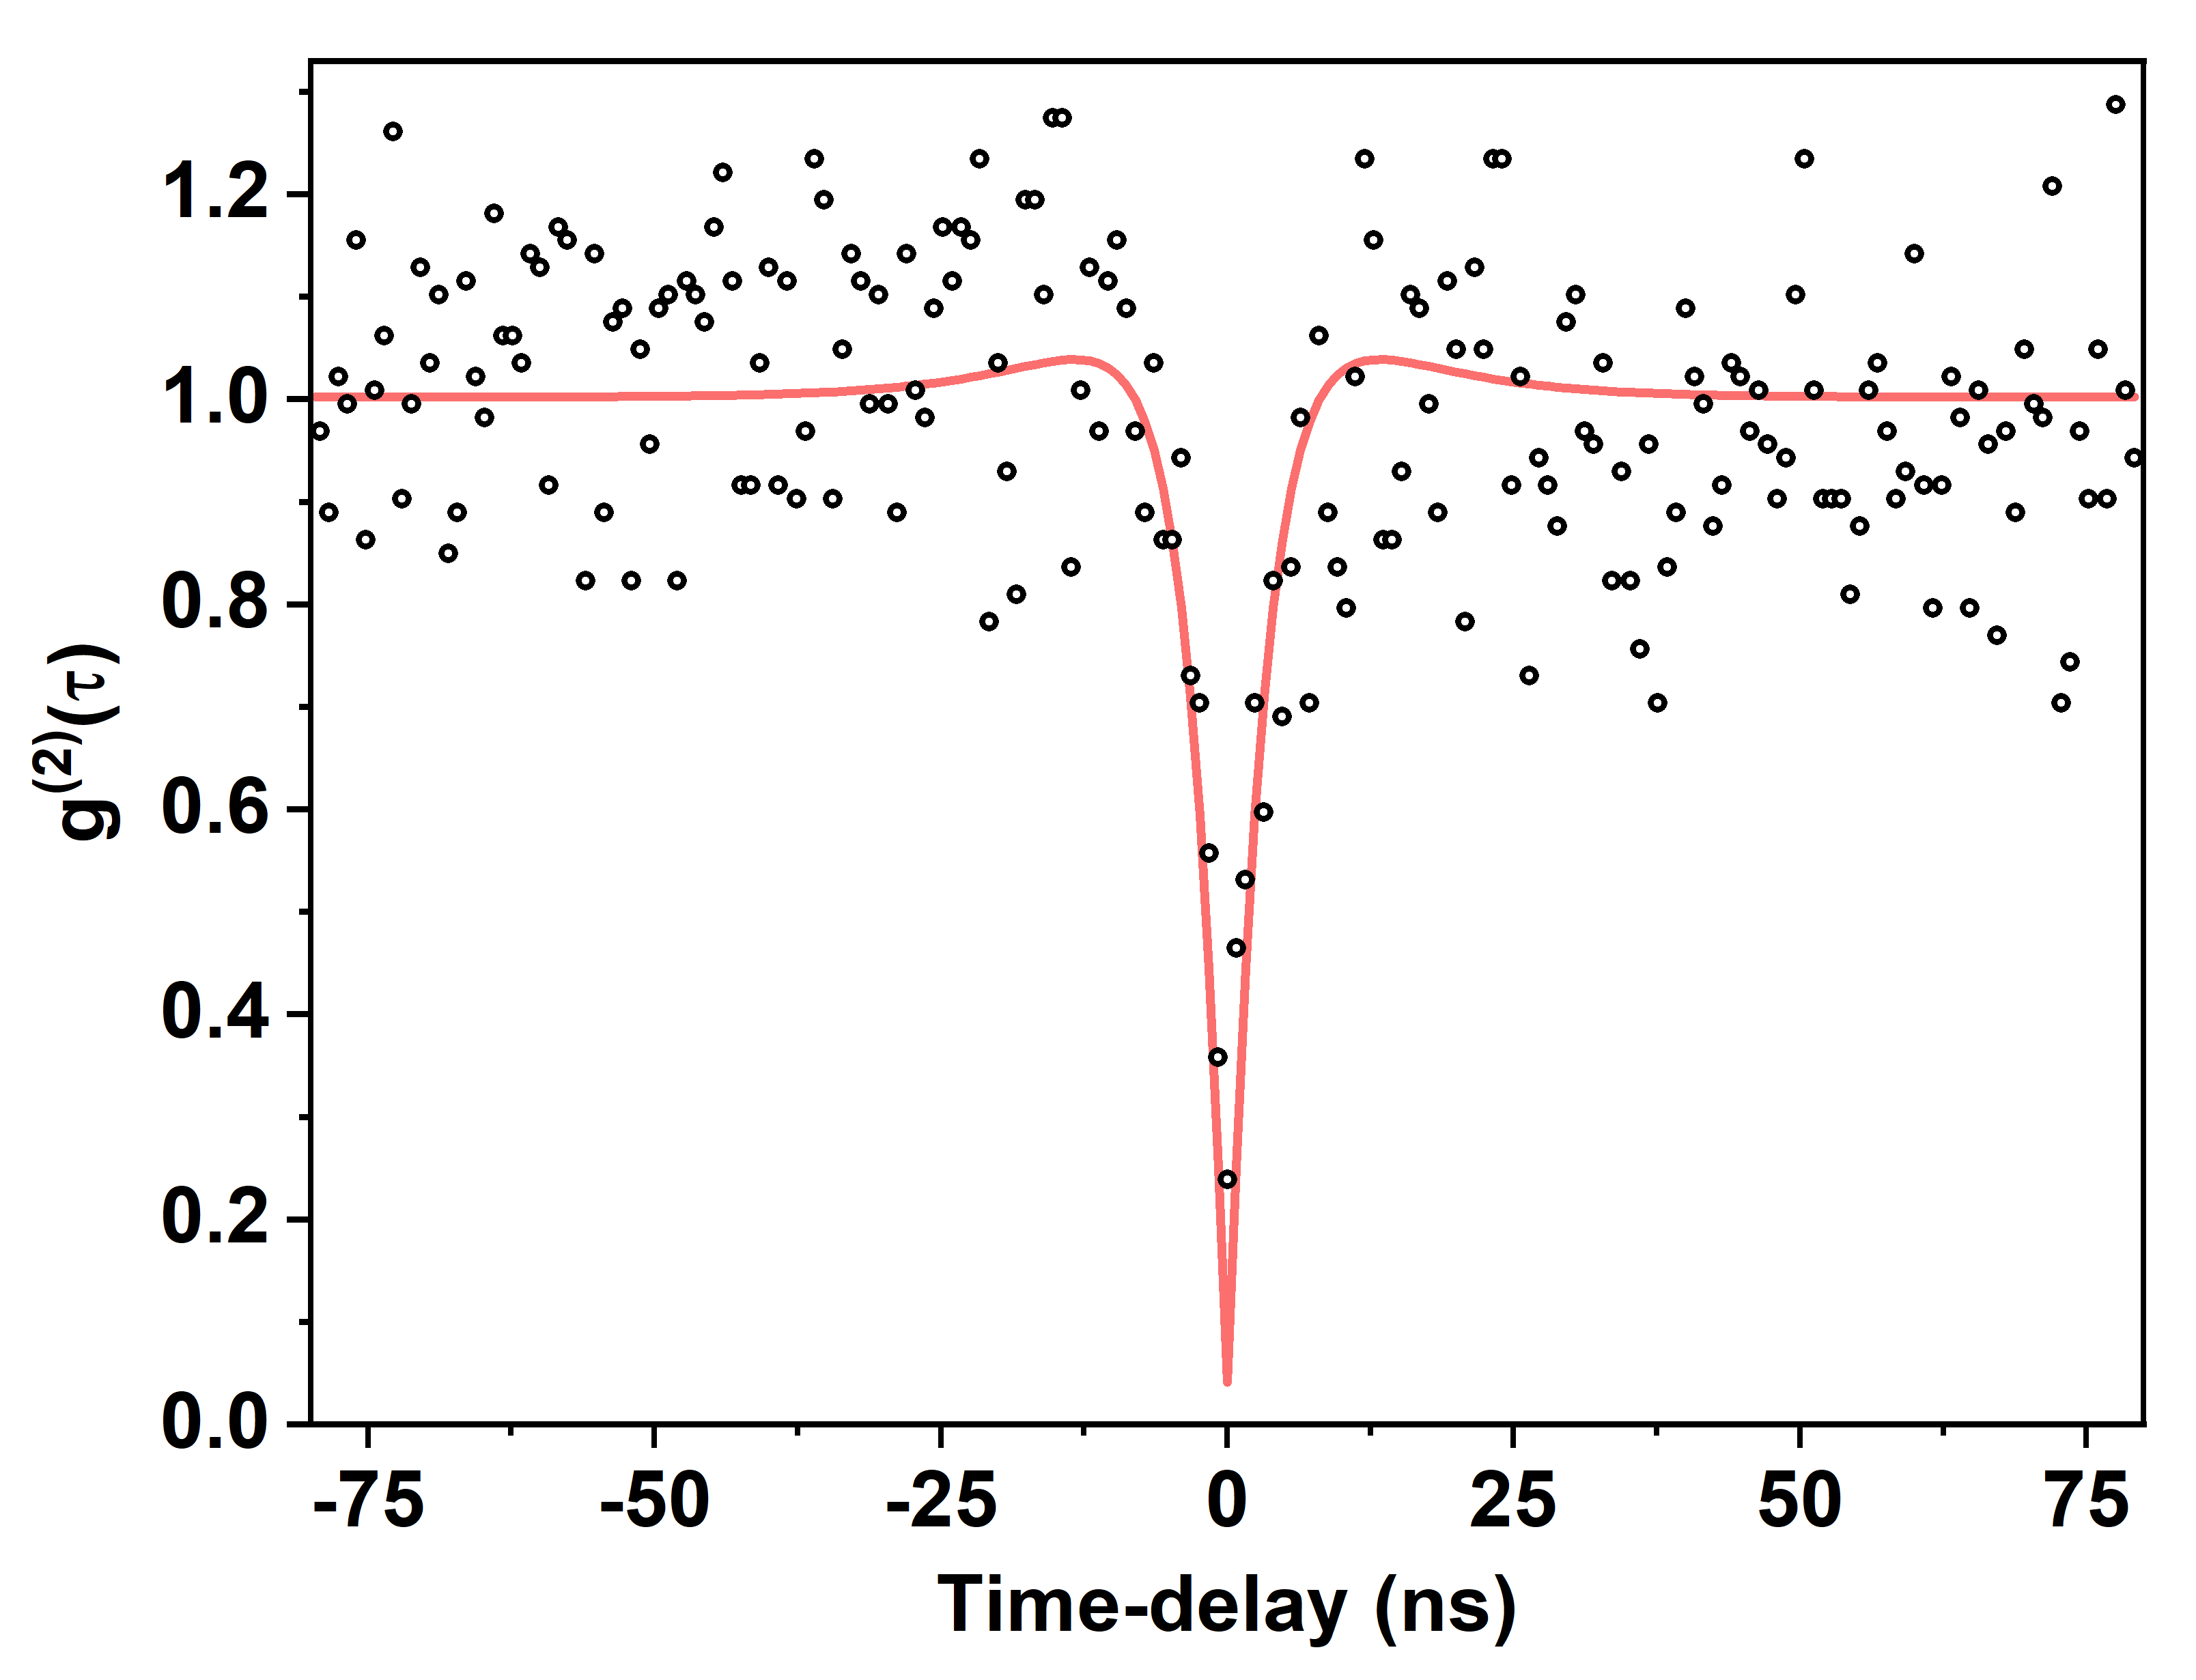
\includegraphics[width=0.85\linewidth]{g2 measuerment.png}
    \caption{Normalized second-order correlation function $g^{(2)}(\tau)$ as a function of time-delay $\tau$ for a single colloidal CdSe QD. Experimental data ($\circ$) is fitted to eq. (\ref{eq:gtwo}) (red curve). The value of $g^{(2)}(0)$ less than 0.5 indicates the presence of a single quantum emitter inside the confocal volume.}
    \label{fig:g2 measurement}
\end{figure}

The second-order correlation function is calculated for 83 particles, of which 64 particles resulted in $g^{(2)}(0) < 0.5$, implying a highly reproducible single-photon emission from the CdSe QDs in the film. The value of $g^{(2)}(0)$ ranges from 0.03 to 0.22. Those particles that lead to $g^{(2)}(0) > 0.5$ might have a size larger than 11.2 nm \cite{MM} which is the exciton Bohr diameter of CdSe. This size corresponds to a weaker confinement of excitons, with a higher probability of multiple-photon emission.



\subsection{Particle-size and radiative lifetime}
The samples used to study single-photon emission in this work are thin films containing CdSe QDs in PMMA prepared via the same procedure. In Figure \ref{fig:size histogram}, we plot the size distribution of the particles in the film, determined from the scanning transmission electron microscope (STEM) images. The corresponding distribution of single-photon emission lifetimes $t_1$ obtained from the second-order correlation function is presented in Figure \ref{fig:lifetime histogram}. The value of lifetime $t_1$ ranges from 0.4~ns to 5.2~ns, implying the spontaneous emission rate $\Gamma_{21}$ varying from 0.2~ns$^{-1}$ to 2.5~ns$^{-1}$ at room temperature. 

Theoretically, the rate of spontaneous emission  of photons, $\Gamma_{21}$,  for the transition between the ground (initial) state $|0 \rangle$ and the excited (final) state $|j \rangle$ is related to the dipole moment matrix elements\cite{AAC}:
\begin{equation}
\Gamma_{21} = {\frac{ \omega_j ^3}{{3 \pi \epsilon_0 \hbar c^3}}| \langle 0| \textbf{D}|j \rangle| ^2}. 
\label{eq:spontan vaccum}
\end{equation}
If  \textbf{r} is the displacement vector pointing from the negative charge (electron) to the positive charge (hole) and $e$ is the unit charge, $\textbf{D} = e \cdot \textbf{r}$ is the dipole moment that characterizes the strength of interaction between the electron and the surrounding medium.  $ \langle 0| \textbf{D}|j \rangle$ refers to the transition dipole moment between the states $| 0 \rangle$ and $|j \rangle$. 

The above expression is valid for the spontaneous emission rate of photons from quantum dots in vacuum. For quantum dots embedded in a matrix, as is the case here, \cite{AAP} the spontaneous emission rate depends on the dielectric constant $\epsilon$ of the medium in which it is immersed, and is given by \cite{YY}
\begin{equation}
\Gamma_{21}^{\prime} = n \Gamma_{21} = \frac{9 \epsilon^{5/2}}{(2 \epsilon + \epsilon_{QD})^2} \Gamma_{21},
\label{eq:spontan rate}
\end{equation}
\noindent where $\epsilon_{QD}$ is the dielectric constant of the QD. Thus the rate of  spontaneous emission can be increased by immersing the QDs in a medium of higher dielectric constant. In our work, CdSe QDs are embedded in PMMA, a medium having dielectric constant of $2.2$ \cite{AAN}, resulting in higher emission rates than reported earlier \cite{AAR, AAS}. 

According to eq. (\ref{eq:spontan vaccum}), $\Gamma_{21}$ depends quadratically on the dipole moment, and hence the radiative lifetime of a particular transition is inversely proportional to the size $r$ of the particle. The radiative lifetime $t_1 = k/r^2$ where $k$ is a constant that depends on the emission frequency,
\begin{equation}
k = \frac{3 \pi \epsilon_0 \hbar c^3}{e^2 \omega ^3} \frac{9 \epsilon^{5/2}}{(2 \epsilon + \epsilon_{QD})^2}.
\label{eq:constant}
\end{equation}
Assuming that the dielectric constant of the QDs does not significantly vary over the size range studied, we may compare the lifetime distribution to the particle-size distribution. To this end, we look at the origin of size distribution in the synthesis of CdSe QDs \cite{FF}. 
After rapid injection of the selenium precursor into the cadmium precursor,  CdSe nuclei are formed and are homogeneously distributed throughout the solution. These sites have the affinity to attract further molecules due to a greater surface-to-volume ratio and grow rapidly to form QDs. Larger clusters above the critical size ($\approx 2$~nm) attract more molecules, while smaller clusters redissolve. Above the critical size, the smaller particles tend to grow much faster due to a large surface-to-volume ratio (and hence, a higher net charge on the surface). The further growth of larger particles slows down because of  insufficient thermal energy to attract further molecules. Hence, the particle-size distribution is skewed towards the smaller particles and a log-normal distribution is favored \cite{AAQ}.
If \textit{r} is particle diameter obtained randomly from STEM image, the probability that \textit{r} takes a range of possible outcomes \textit{R} (such that \textit{r} $\in$ \textit{R}) has  a log-normal probability density function given by
\begin{equation}
    P_r(R) = \frac{1}{R \sigma \sqrt{2 \pi}} exp \Biggl \{- \frac{(\ln(R)- \mu)^2}{2 \sigma^2} \Biggr \},
    \label{eq:size distribution}
\end{equation}
with mean  $\mu$ and standard deviation $\sigma$  of the logarithmic values of the random sizes \textit{r}. The solid red line in Figure \ref{fig:size histogram}, is a log-normal fit to the size distribution with R-squared value of 0.88.

\begin{figure}
    \centering
    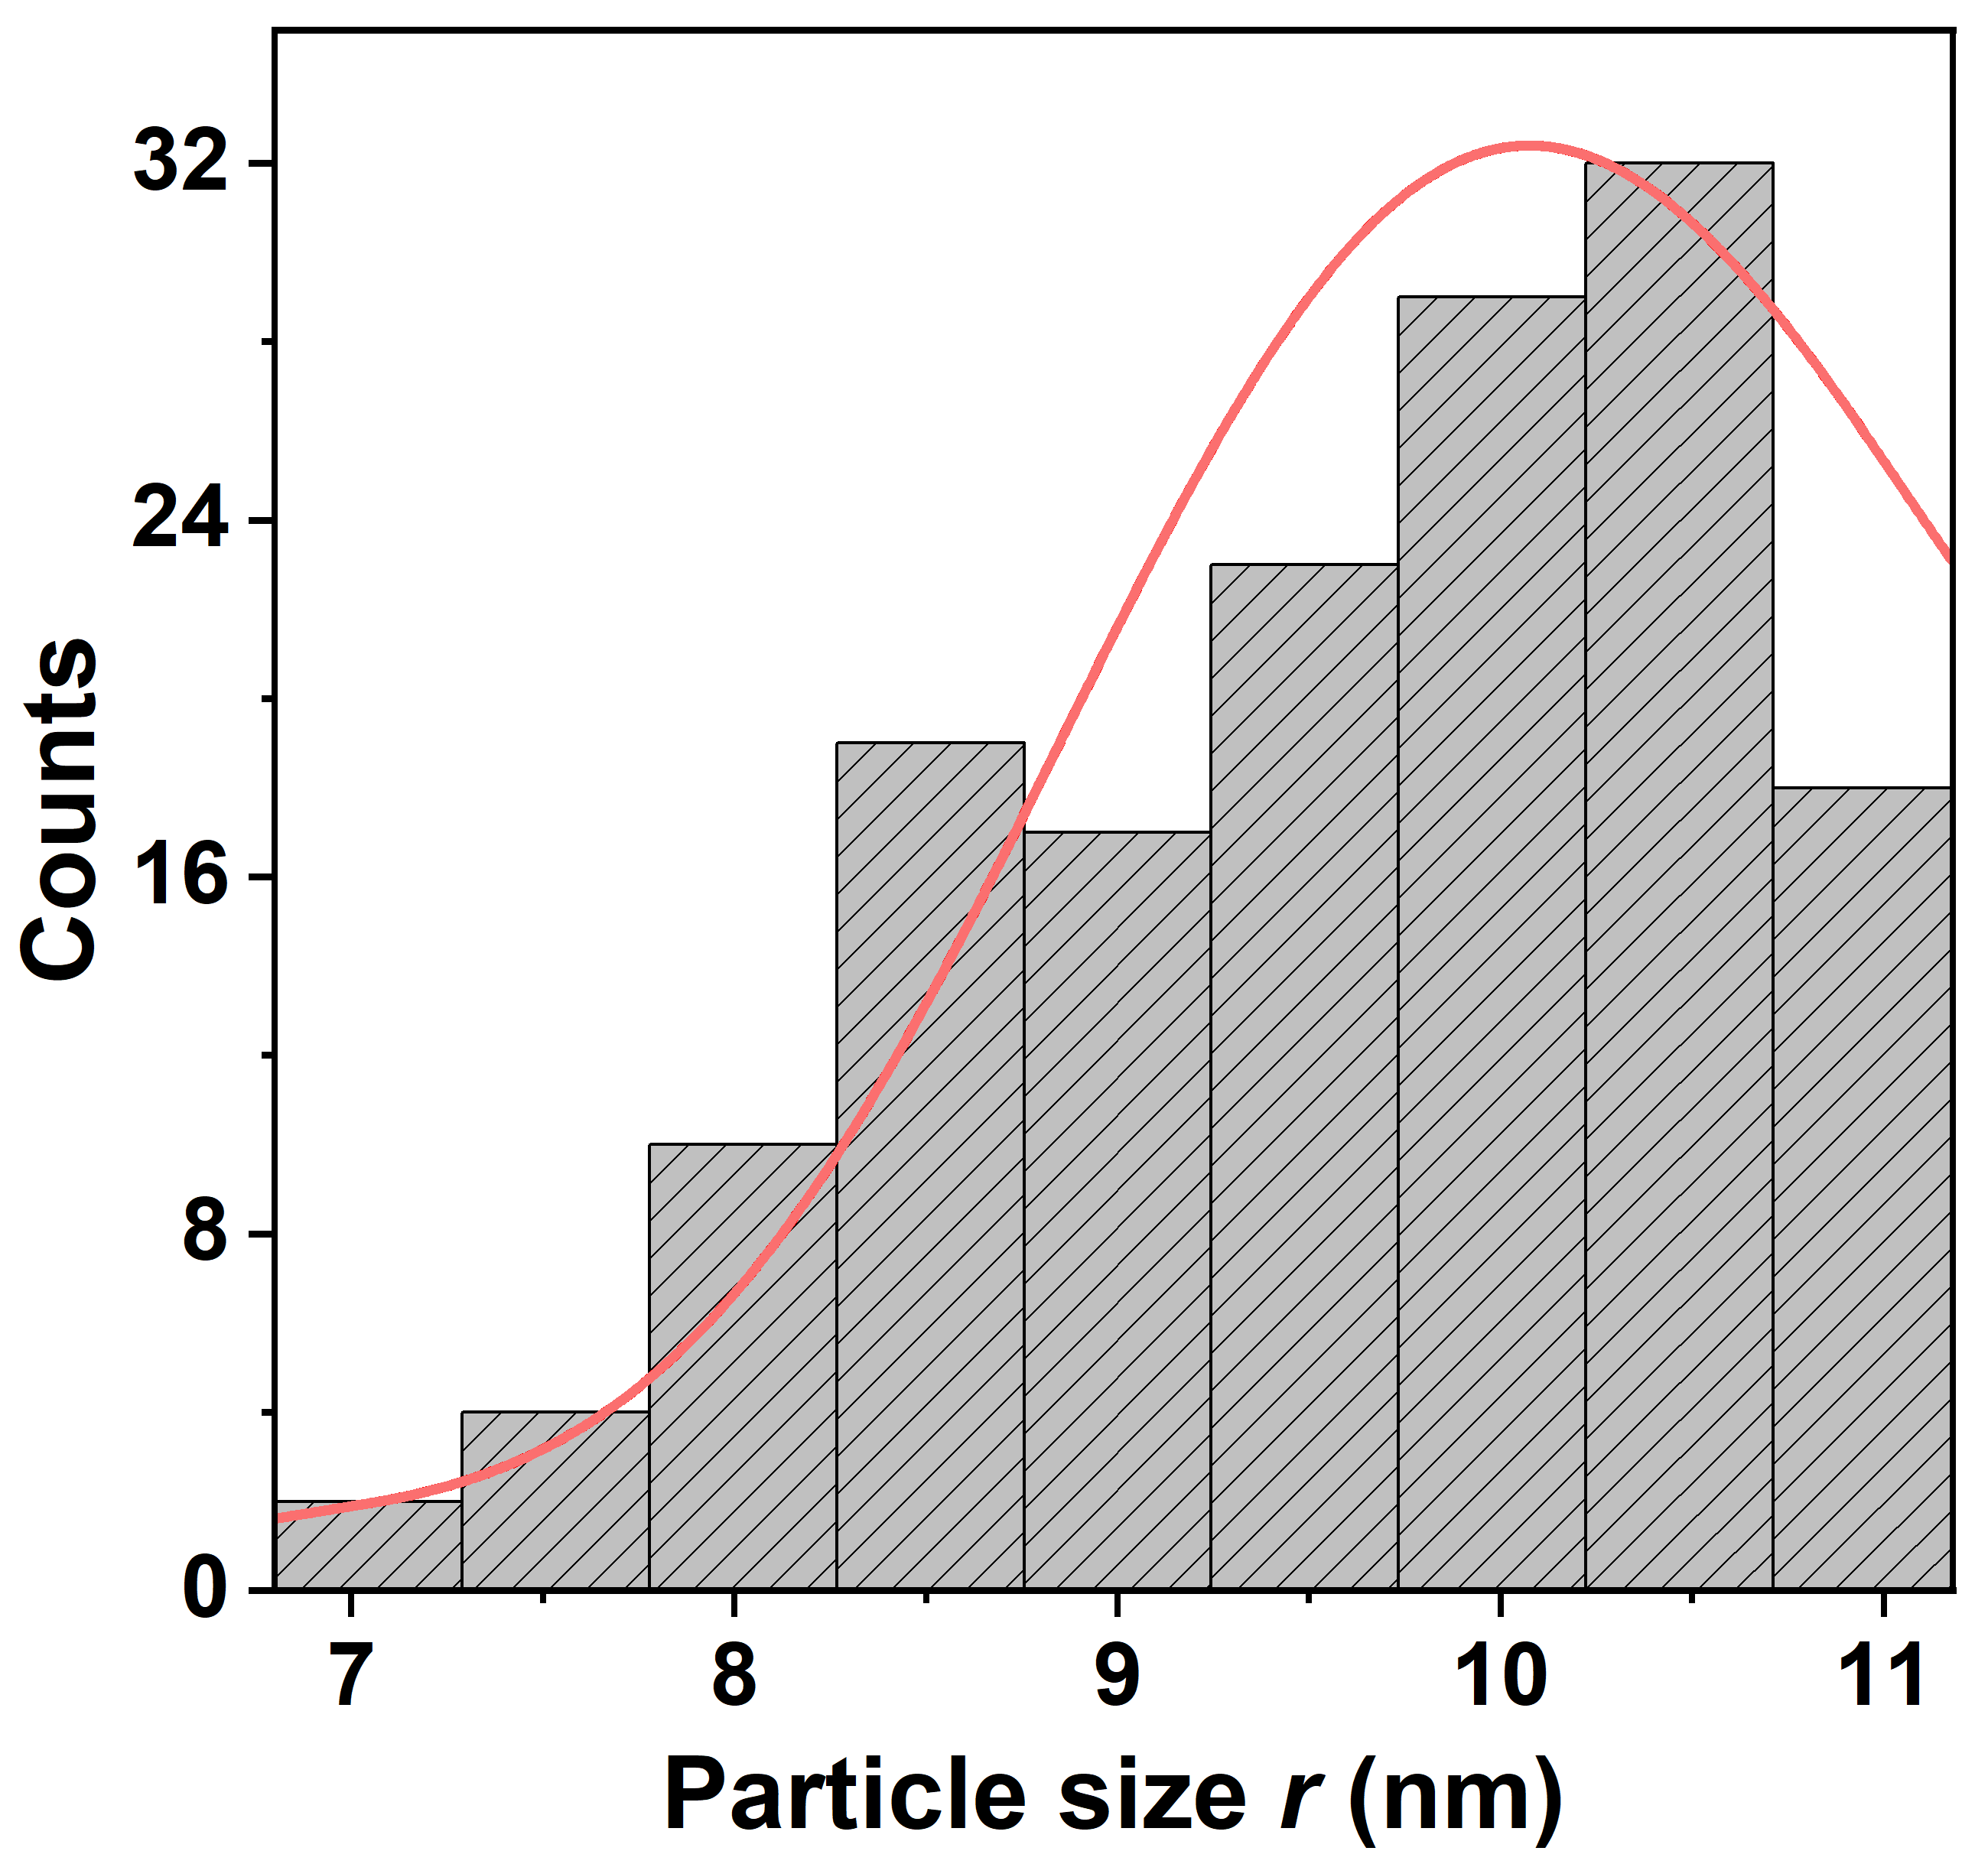
\includegraphics[width=0.8\linewidth, height=0.7\linewidth]{histogram of size.png}
    \caption{Particle-size (diameter) distribution obtained from STEM image for size up to 11.2~nm (exciton Bohr diameter). This distribution is fitted using log-normal probability density function of Eq \eqref{eq:size distribution}, shown by the red curve.}
    \label{fig:size histogram}
\end{figure}

\begin{figure}
    \centering
    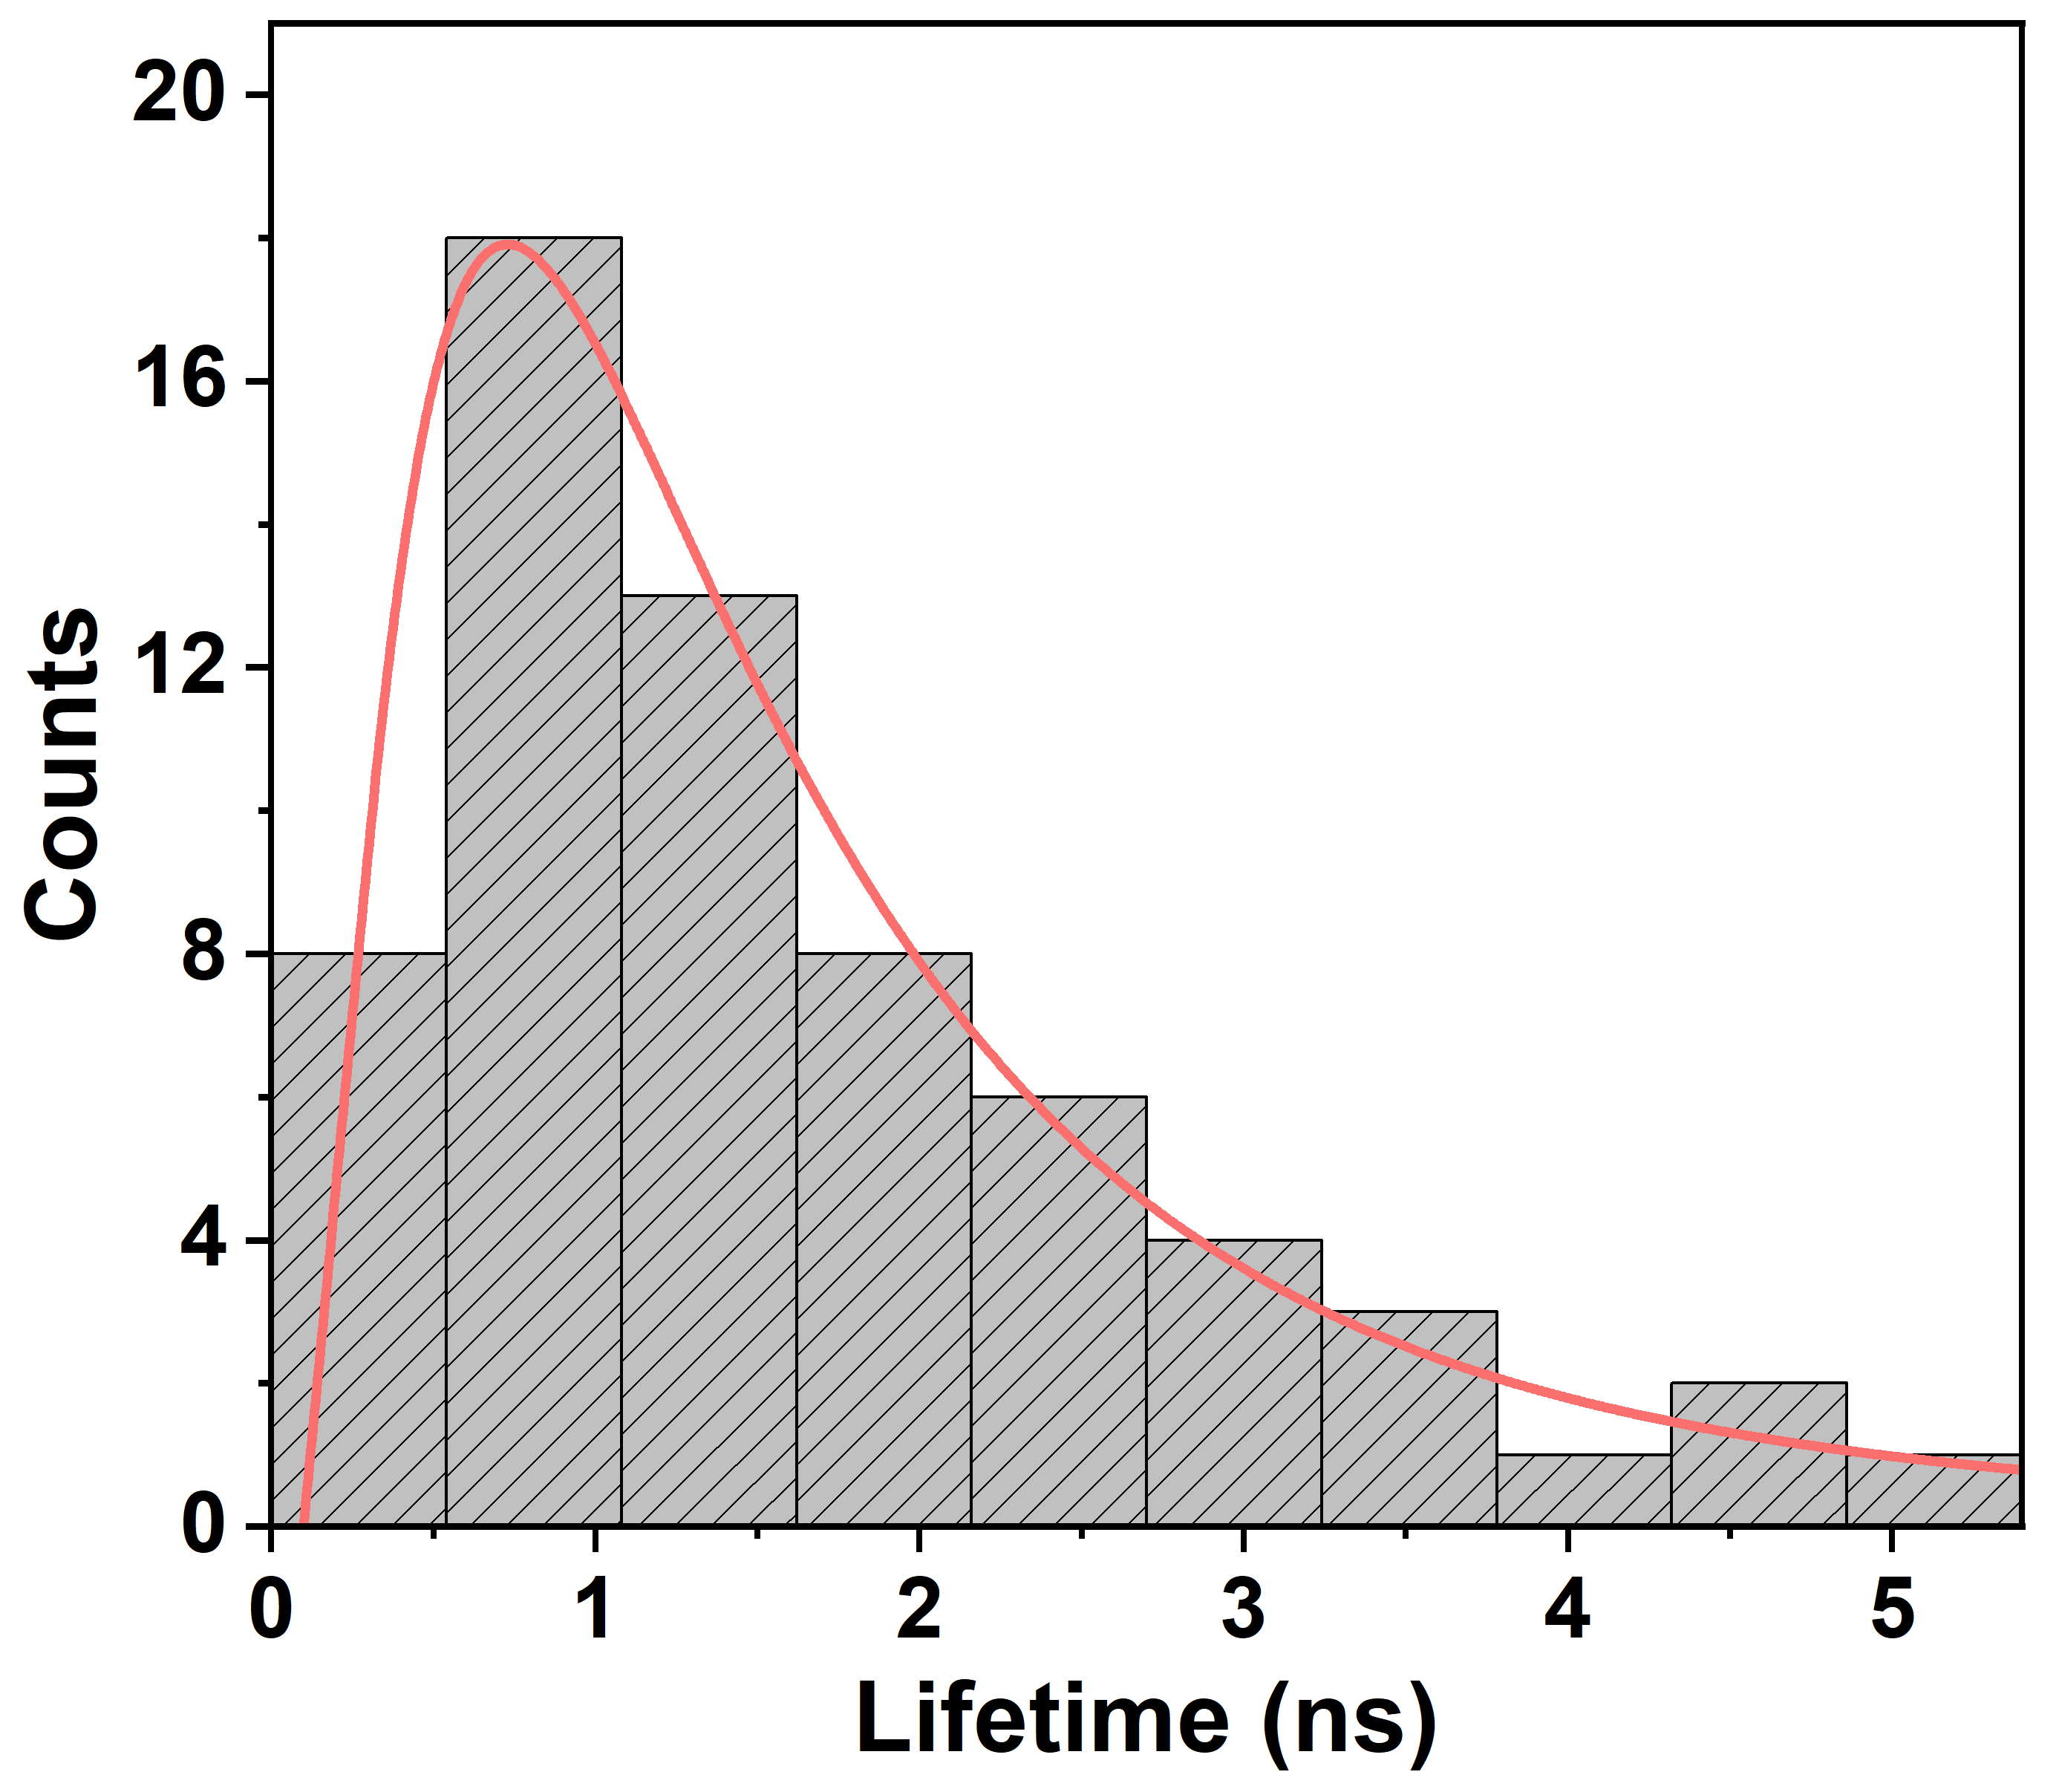
\includegraphics[width=0.8\linewidth, height=0.7\linewidth]{histogram of lifetime.png}
    \caption{Distribution of single-photon emission lifetimes ($t_1$) of the CdSe QDs at 650~nm obtained from the second-order correlation function. Only the correlation data with $g^{(2)}(0) < 0.5$, representing single-photon emission, is considered here. The lifetime distribution is fitted (red curve) with the function given in eq. (\ref{eq:lifetime distribution}).} 
    \label{fig:lifetime histogram}
\end{figure}


Since the radiative lifetime $t_1 = k/r^2$, the lifetime distribution has a probability density function given by 
\begin{equation}
    P_{t_1}(T_1) = \frac{1}{2T_1 \sigma'  \sqrt {2 \pi}} exp \Biggl \{- \frac{(B - \ln(T_1))^2}{8 \sigma'^2} \Biggr \}
    \label{eq:lifetime distribution}
\end{equation}
where $B=\ln(k) - 2\mu$ is the mode of the distribution.  In Figure \ref{fig:lifetime histogram}, the lifetime distribution is shown along with a fit to the log-normal distribution. The R-squared value of the fit is 0.99, indicating a good agreement with eq. \ref{eq:lifetime distribution}. An exciton in a larger QD exhibits a larger optical dipole moment when compared to a smaller QD. A consequence of having a large optical dipole moment is the rapid decay of excitons \cite{MM}, leading to a shorter lifetime. The lifetime distribution in Figure \ref{fig:lifetime histogram} may be compared with the size distribution in Figure \ref{fig:size histogram}. The size distribution  peaks at 10.5~nm, while the lifetime distribution has its peak at $\approx$ 0.8~ns. From a comparison of these two distributions, we may infer that lifetimes lower than that of 0.8~ns are exhibited by particles having a size larger than 10.5~nm.

Strong confinement of carriers in CdSe QDs would occur below the exciton Bohr diameter, which is approximately equal to 11.2~nm \cite{MM}, beyond which the probability of multiple-photon generation is high. Hence, a distribution of particle size up to 11~nm is shown in Figure \ref{fig:size histogram} for  comparison with the lifetime distribution. It is noticed that the lifetime is negatively correlated with the size of the particle. 

The strength of the monotonic relationship between the particle size and the radiative lifetime is assessed by Spearman's rank correlation coefficient $\rho$, which takes the values $(-1 \leq \rho \leq +1)$, where +1 corresponds to perfect positive correlation, and -1  to perfect negative correlation. The value zero indicates the absence of any correlation. To calculate $\rho$, the curve fitting functions for the size ($r$) distribution and the lifetime ($t$) distributions are discretized into 100 data points.  The discrete data points for both size and lifetime distributions exhibit one-to-one correspondence through the relation $t_1 = k/r^2$. If $d_i$ is the difference between the ranks of the $i^{th}$ pair of values of $r$ and $t$, and $n$ is the largest rank, then the Spearman rank correlation coefficient is calculated using 
\begin{equation}
    \rho = 1 - \frac{6}{n(n^2 -1)}\sum d_i^2. 
\end{equation}
For the present data, $\rho$ is estimated to be  $-0.749$, which indicates that the particle size and radiative lifetime are negatively correlated.

The good correlation between the size distribution and the lifetime distribution may prompt us to hazard an estimate of the constant $k$ in the relation $t_1 = k/r^2$. We can safely assume that the peak value seen at 0.8 ns in the lifetime distribution corresponds to particles of size 10.5 nm, where the maximum number of particles are observed in the size distribution, within the error limits of our bin width. This tells us that the value of $k$ is equal to $(9 \pm 3) \times 10^{-26}$. This analysis shows that the sizes of the quantum dots studied by us vary from $(14 \pm 2)$ nm (for an excited state lifetime of 0.4 ns) to $(4.1 \pm 0.6)$ nm (for an excited state lifetime of 5.2 ns).

\begin{figure}
    \centering
    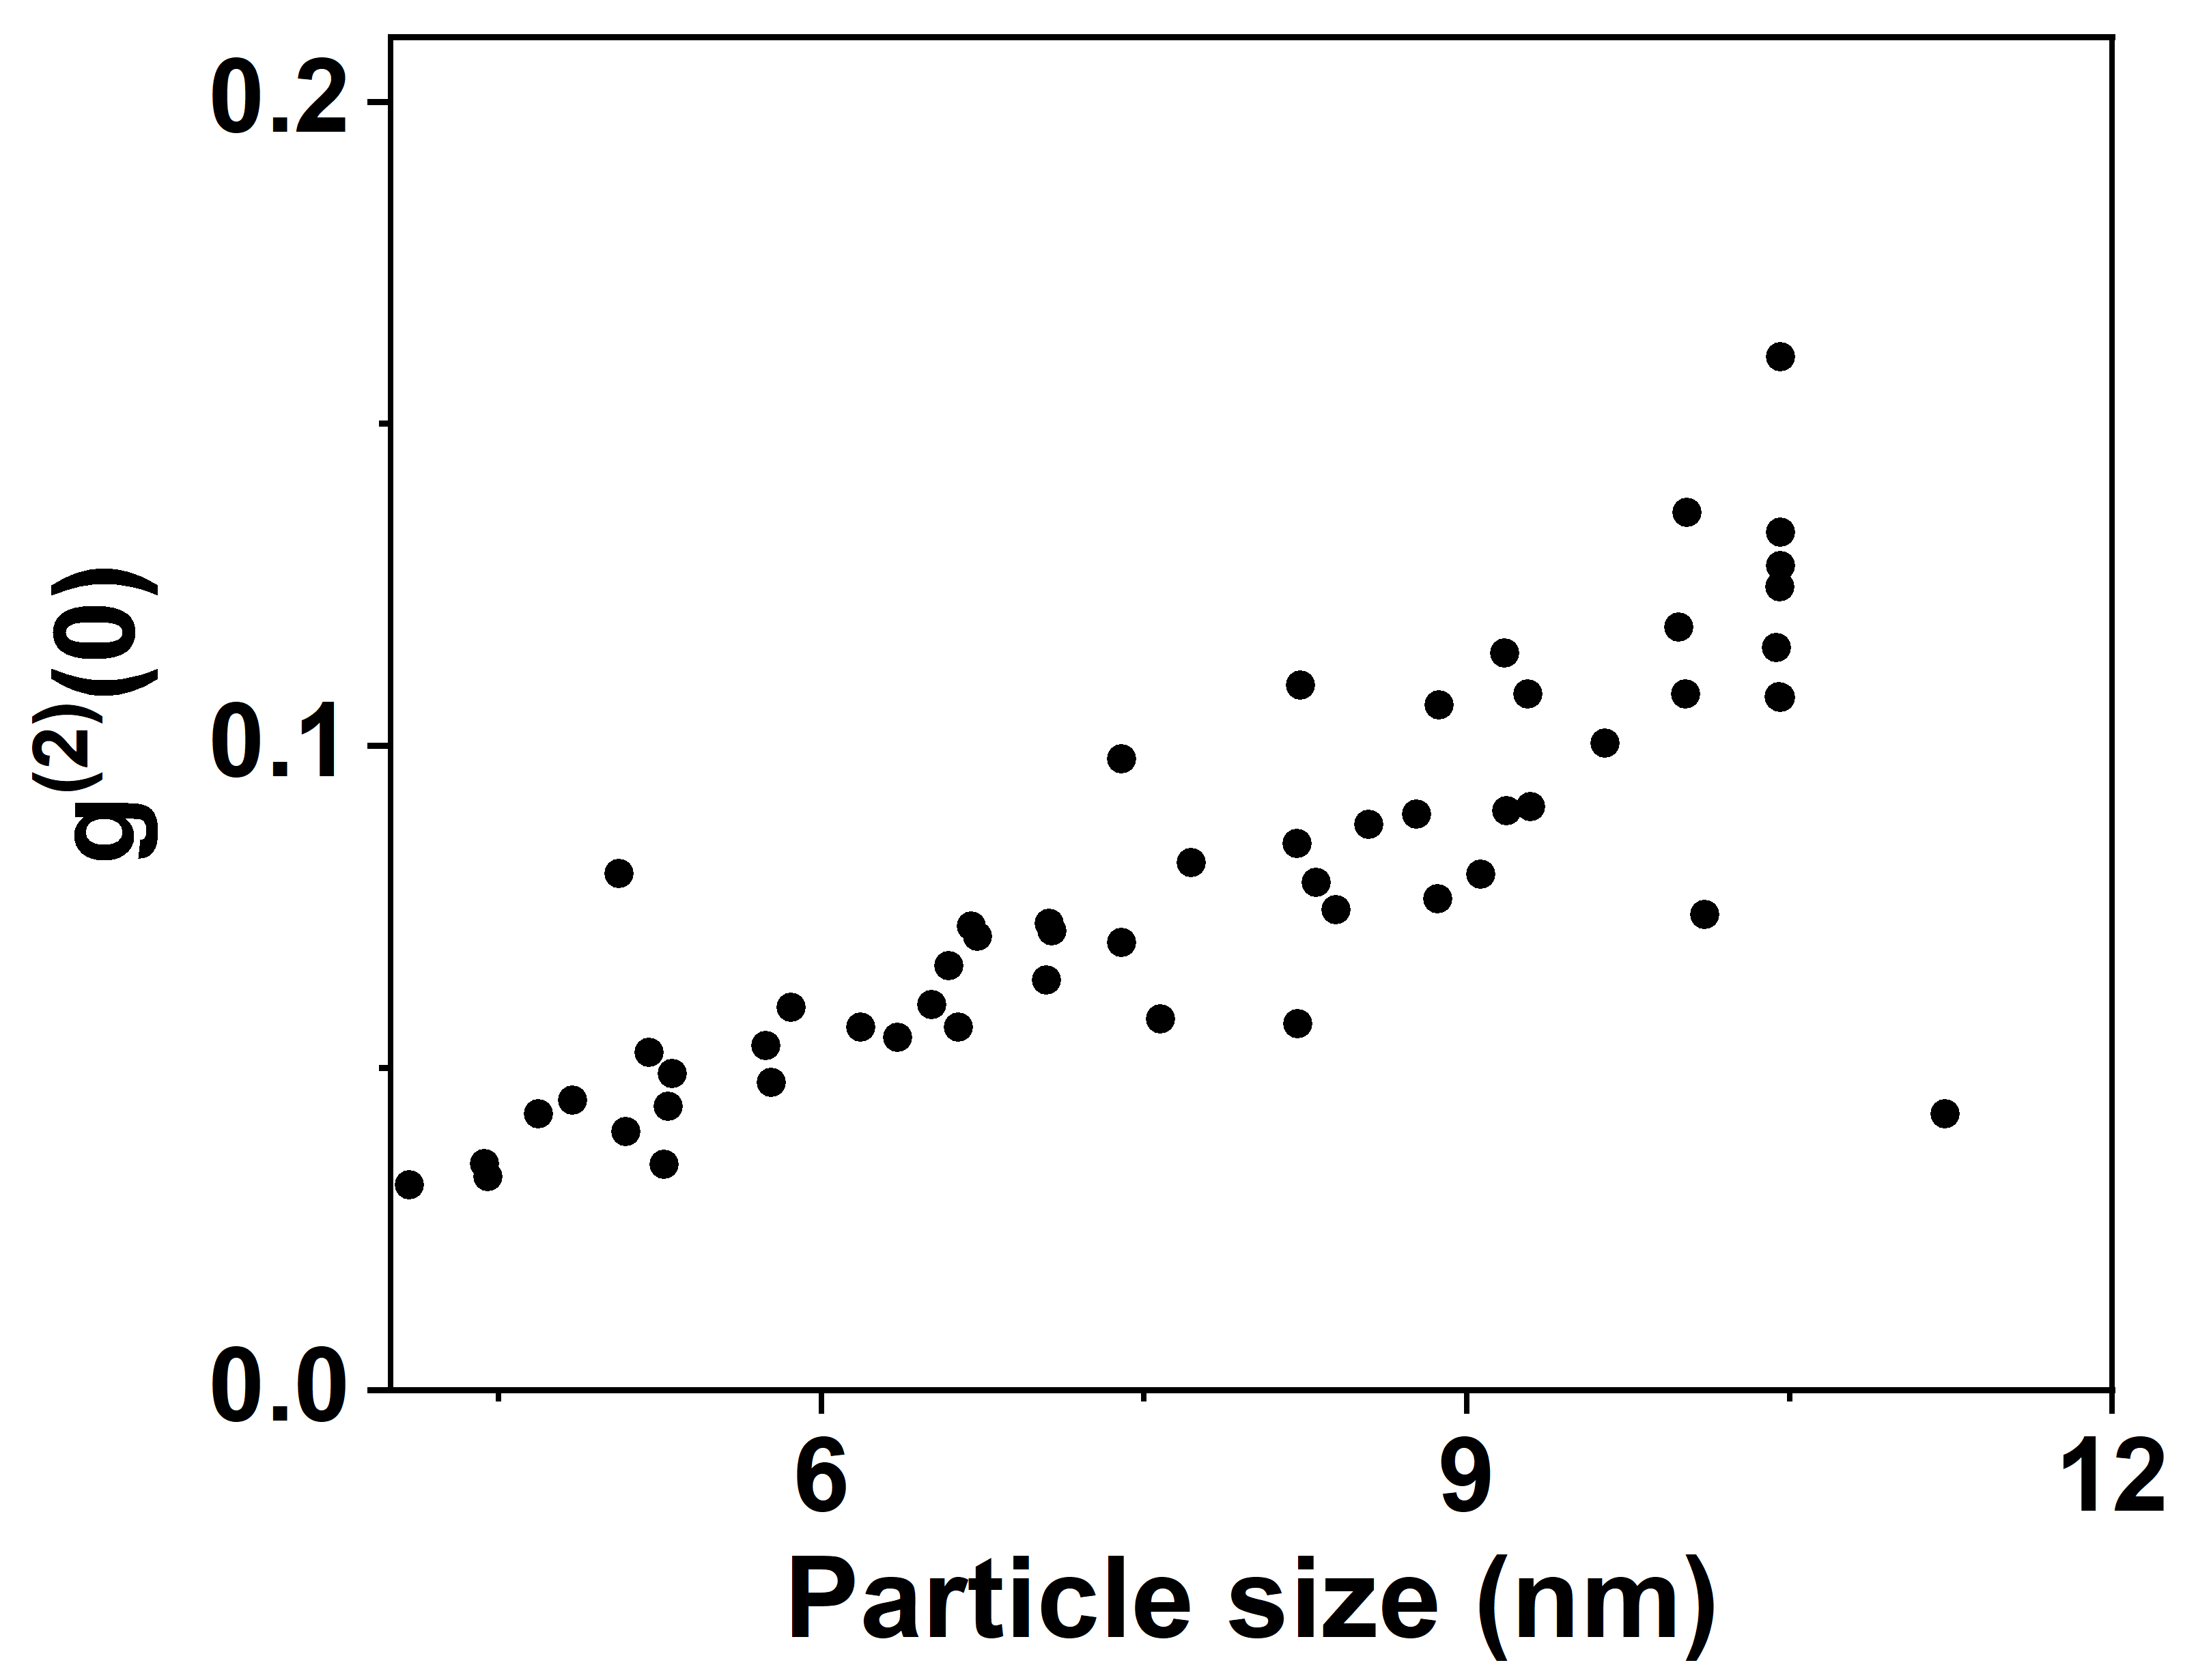
\includegraphics[width=0.65\linewidth, height=0.55\linewidth]{g2 vs size1.png}
    \caption{Plot of $g^{(2)}(0)$ obtained using HBT experiment versus size obtained using $r = \sqrt{k/t_1}$. Single photons are emitted from the particles in the confinement regime, hence $g^{(2)}(0) < 0$. The probability of multiple-photon emission increases with increase in the particle-size and it results in increase in $g^{(2)} (0)$.}
    \label{fig:correlated size and lifetime}
\end{figure}

Estimating the size of nanoparticles embedded in dielectric films is important for different experiments and applications. However, optical imaging does not have the resolution to determine the size of nanoparticles in the size range below the diffraction limit. Estimating the size of these particles is a major challenge due to the special sample preparation techniques needed for electron microscopes. A monotonic relationship between the particle size distributions of identically prepared nanoparticles and their optical absorption properties has been established elsewhere \cite{AAT}.
Due to the strong correlation between particle size and radiative lifetime, the method discussed above could be a promising approach to estimating the size of nanoparticles embedded in a thin film using optical methods. 
In Figure \ref{fig:correlated size and lifetime}, we plot $g^{(2)} (0)$ for the particles studied against the estimated size. The plot shows that $g^{(2)} (0)$ increases with size and also that there is a large fluctuation in the value of $g^{(2)} (0)$ for particle sizes above exciton Bohr diameter of 11.2 nm. This behavior further demonstrates the fact that the probability of multiple-photon emission increases with increasing particle size. 



\section{Summary and Conclusion}
In this work, we study the single-photon emission characteristics of monodisperse colloidal CdSe QDs synthesized using a green synthesis protocol. The radiative lifetime of these QDs is estimated by analyzing the second-order correlation function $g^2(\tau)$ measured using an HBT setup attached to an in-house constructed confocal microscope. An order of magnitude increase in the single-photon emission rate is achieved by embedding CdSe QDs of size close to the exciton Bohr radius in a medium having a high dielectric constant. Embedding the QDs in a medium results in a weak overlap of the electron (hole) wave function at the QD-medium interface, thereby reducing the radiative lifetime. The value of $g^2(0)$ ranging from 0.03 to 0.22 at room temperature for 64 trials out of 83 trials indicates high-quality single-photon emission. By comparing the CdSe QD size distribution with the lifetime distribution, we could qualitatively estimate the size of the CdSe QDs from their single-photon emission lifetime. From this analysis, we could determine the value of $g^2(0)$ as a function of QD size, and it is observed that $g^2(0)$ increases with QD size. A larger spread is observed in the $g^2(0)$ values as the size of the QD increases. This observation is supported by the fact that there is a larger probability of multiple-photon emission as the QD size increases. 


\begin{acknowledgments}
We want to acknowledge Martin Kernbach from Johannes Kepler University, Linz for useful discussions on experimental setup and second-order correlation function. We are thankful to Nehal Waghchoure from the Department of Chemistry for the discussions on the synthesis process and Abhishek Yadav from the Department of Mathematics for assistance in creating the Matlab algorithm. The authors would also like to acknowledge Arun V. Kulkarni and Chandradew Sharma, Department of Physics for the discussion on evaluating the distribution function. We are grateful to the Central Sophisticated Instrumentation Facility (CSIF) of BITS Pilani for the assistance with the STEM imaging and photoluminescence spectrum of quantum dots.  We also acknowledge the support by the Department of Science and Technology, Govt. of India under the DST-FIST scheme (Ref No. SR/FST/PSI-142/2009; SR/FST/PS-I/2017/21).
\end{acknowledgments}

\section*{Data Availability Statement}
The Matlab algorithm for the data analysis of HBT experiment is available online in \href{https://github.com/hbtmatlab/g-2-for-photons/tree/main}{GitHub}. All other experimental data related to this study are available from the corresponding author.



\appendix
\section{\textbf{Scanning Transmission Electron Microscopy}}
The thin films of colloidal CdSe QDs are imaged using scanning transmission electron microscopy (STEM) (0.8 nm resolution, FEI Quanta FEG 250) as shown in Figure \ref{fig:CdSe_STEM_image} for size characterisation. A closer observation of individual spots in the image reveals largely monodisperse quantum dots even though a few agglomerated clusters are also present. The fogginess observed in the background of the image is oleic acid used for the synthesis of CdSe QDs. This is confirmed by the photoluminescence peak of oleic acid (435 nm) obtained from the region where CdSe QDs were absent in STEM imaging. The average size of (10 $\pm$ 1) nm from 200 monodisperse CdSe QDs with a polydispersity index of 0.11, indicates a narrow size distribution obtained from heat-up synthesis. Energy-dispersive X-ray (EDX) spectrum shown in Figure \ref{fig:EDX} reveals the composition of various elements in colloidal CdSe QDs film. The appearance of a silicon peak is from the glass substrate and it is prominent due to the very low density of monodisperse CdSe QDs. Carbon and copper peaks arise from the carbon-coated copper grids used for STEM imaging.

\begin{figure}
    \centering
    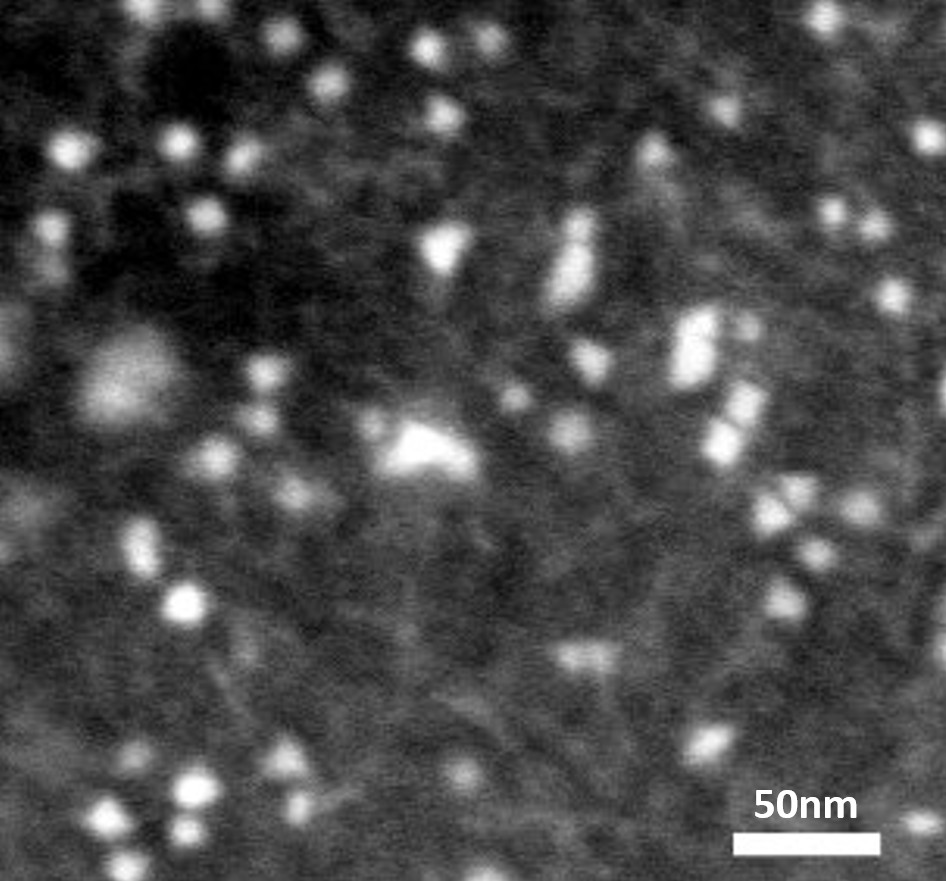
\includegraphics[width=0.7\linewidth]{STEM image CdSe.png}
    \caption{STEM image of colloidal CdSe QDs. Bright spots are the individual particles and the foggy background is the remnant oleic acid. The scale bar is 50 nm. The average size of particles is (10 $\pm$ 1) nm.}
    \label{fig:CdSe_STEM_image}
\end{figure}


\begin{figure}
    \centering
    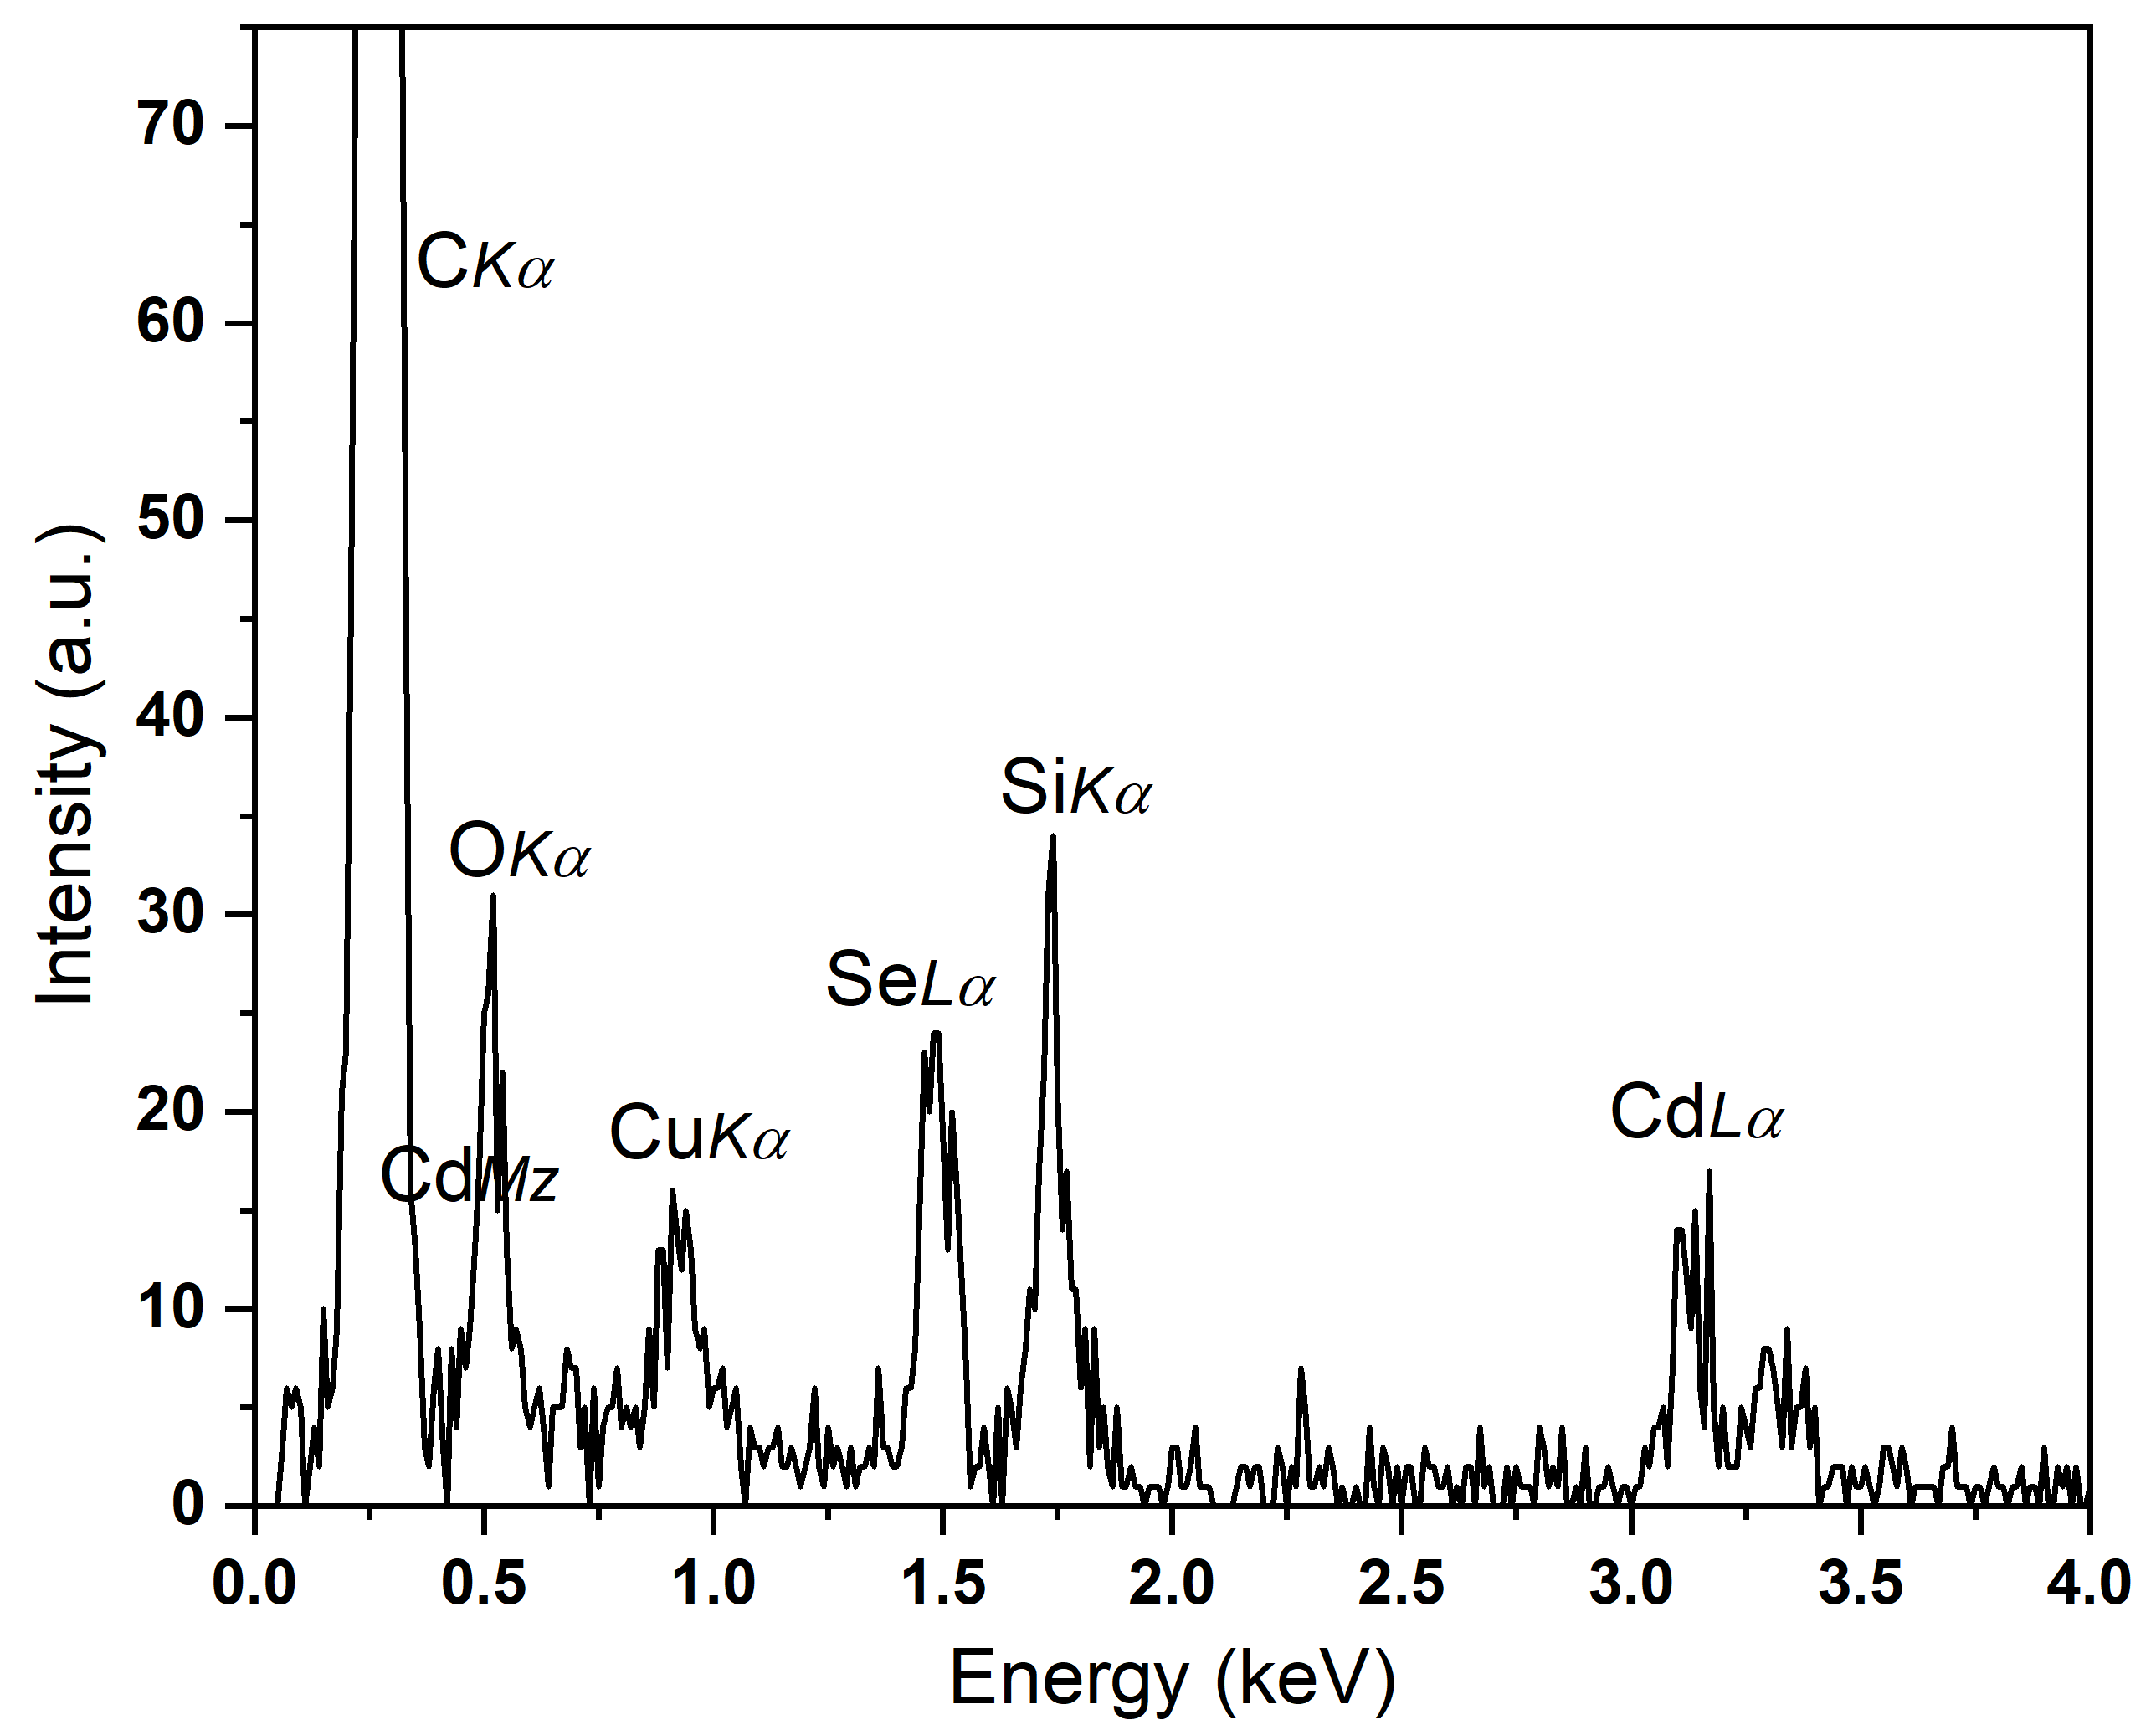
\includegraphics[width=0.8\linewidth]{EDX data.png}
    \caption{EDX data for CdSe QDs sample on a glass substrate. Cadmium and selenium peaks arise from the sample whereas silicon, carbon, copper, and oxygen peaks are from glass, copper grid, and oleic acid.}
    \label{fig:EDX}
\end{figure}


\section{\textbf{Absorption and Photoluminescence spectroscopy}}
Absorption spectra of the colloidal CdSe QDs is studied using UV-Vis spectrometer (V-750, Jasco Inc.) (Figure \ref{fig:optical spectra} (a)). A bandgap energy of 1.95 eV is obtained from the corresponding Tauc plot (inset of Figure \ref{fig:optical spectra} (a)), which is greater than that of the bulk cadmium selenide (1.74 eV). The increase in the bandgap is due to the quantum confinement effects.

\begin{figure}
    \centering
    \subfigure{(a)}{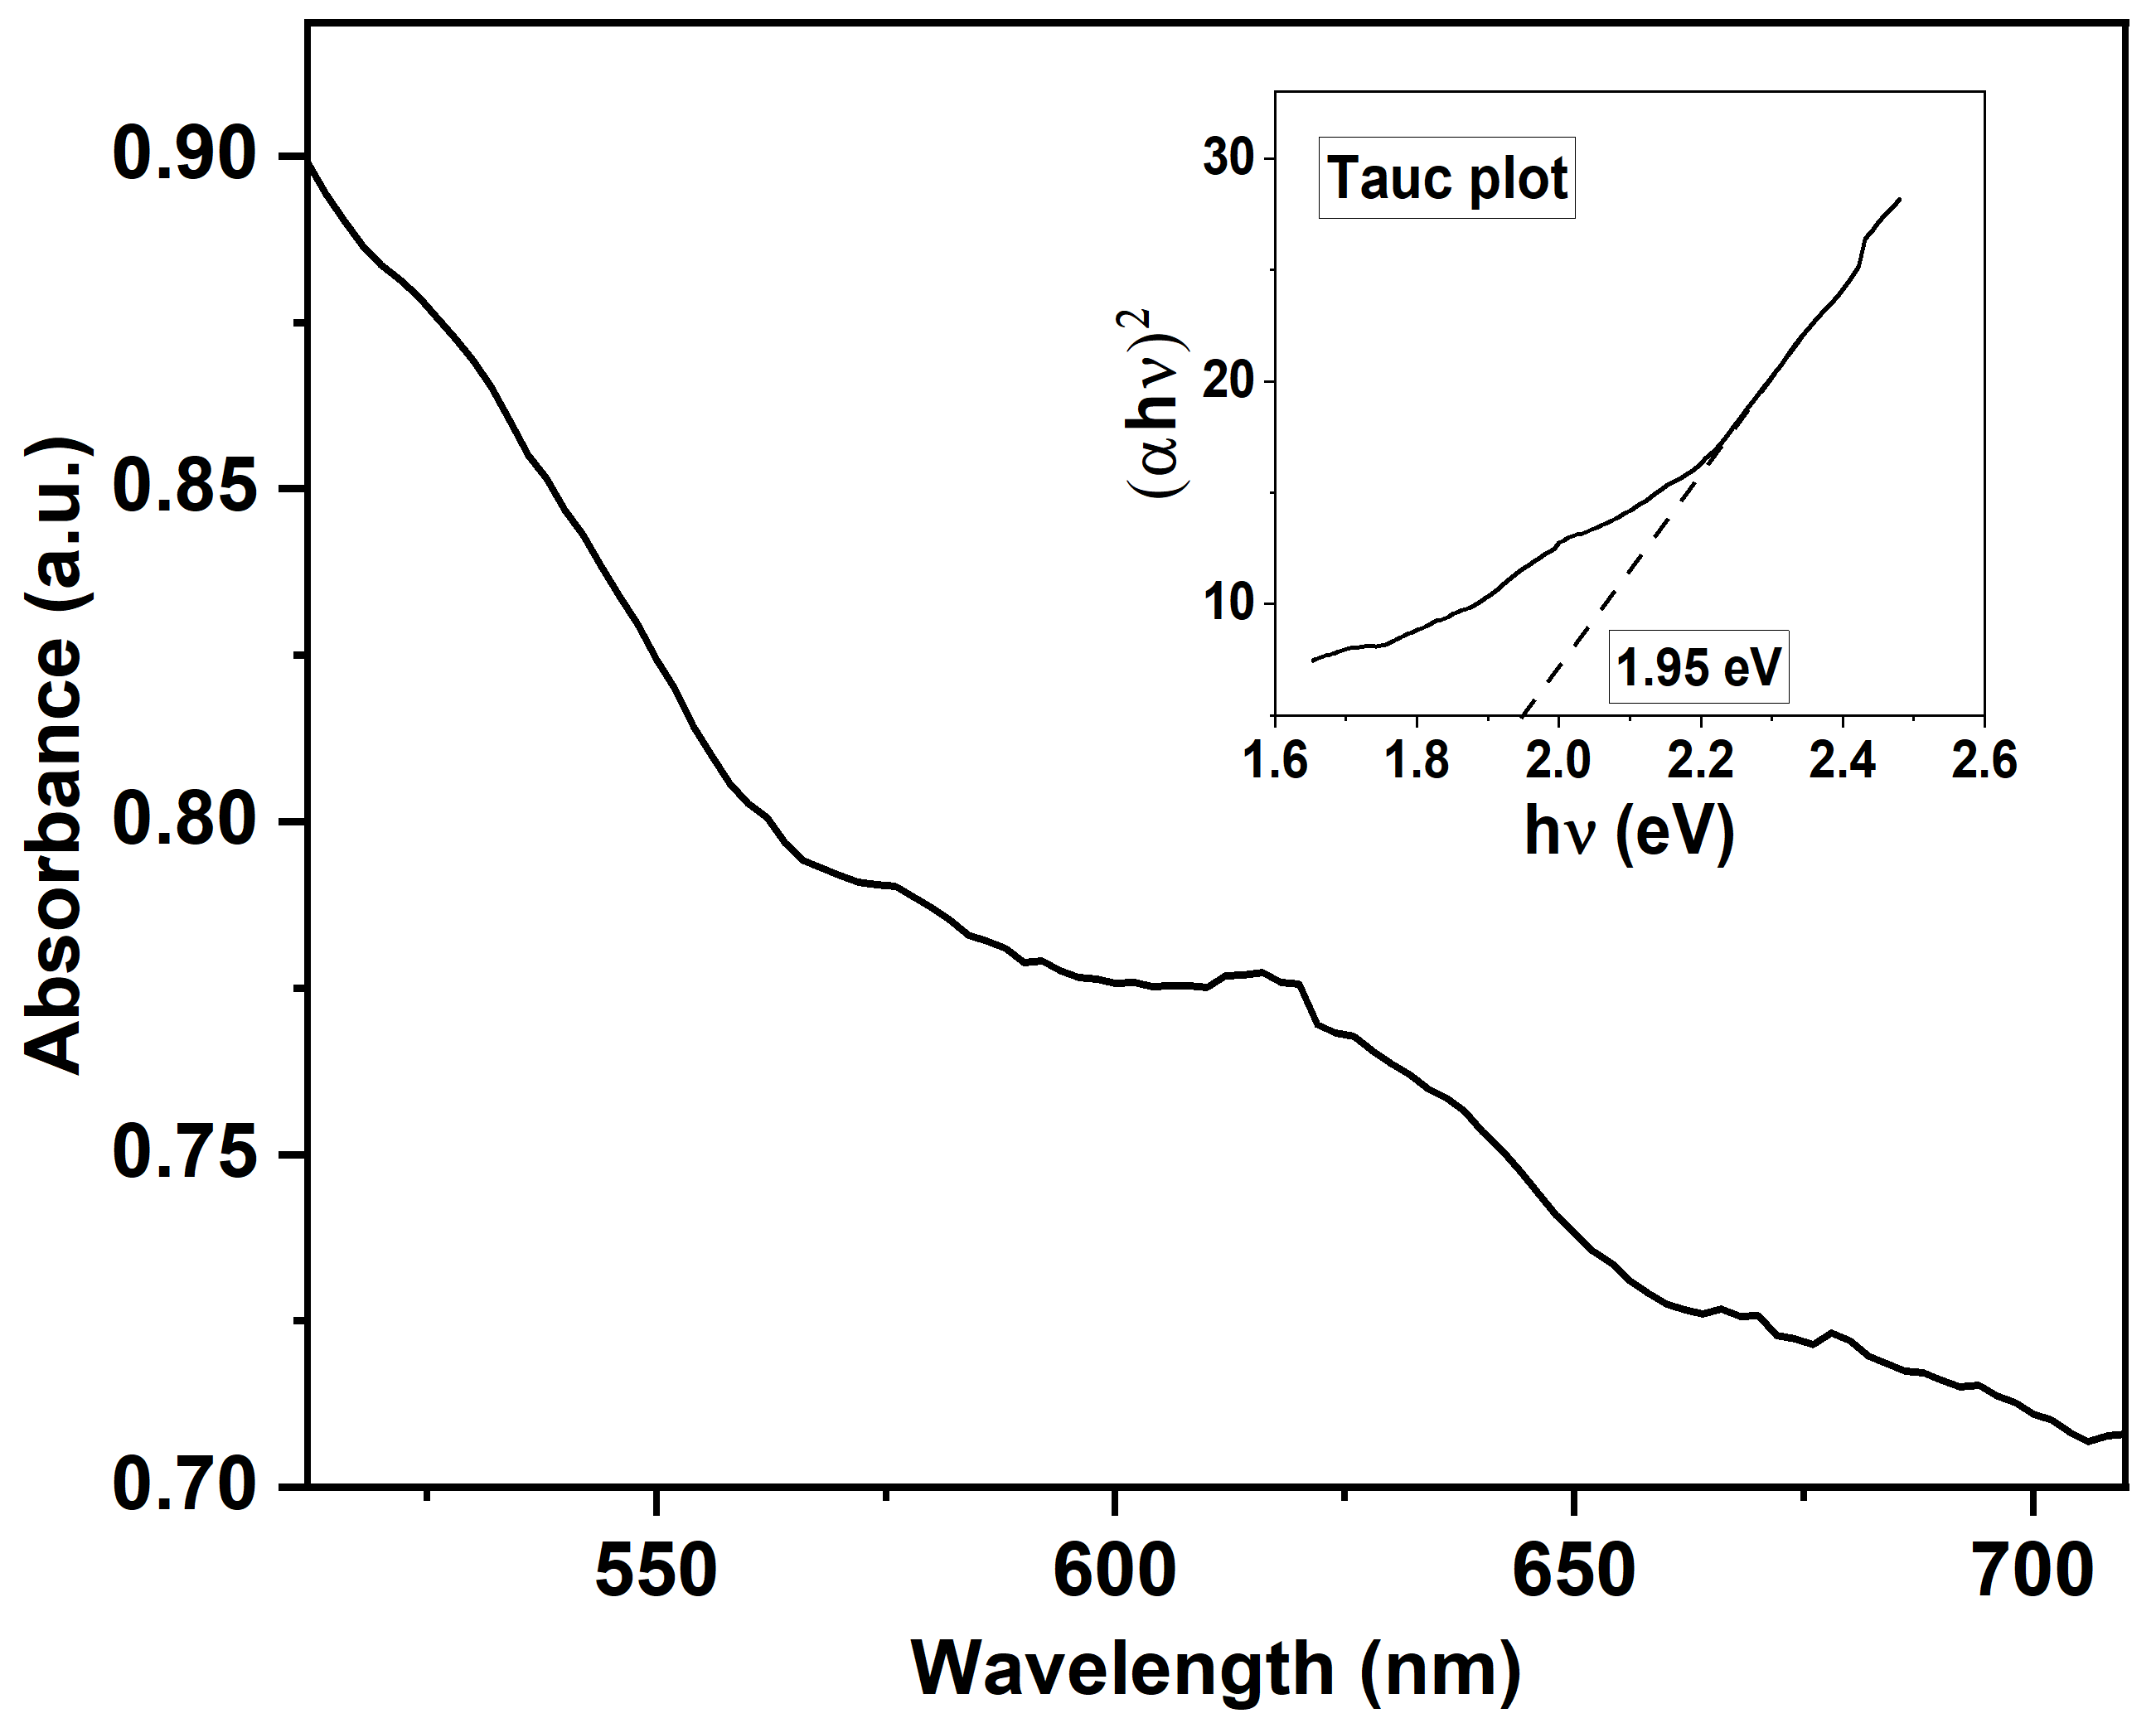
\includegraphics[width=0.74\linewidth]{Absorption spectrum.png}}
    \subfigure{(b)}{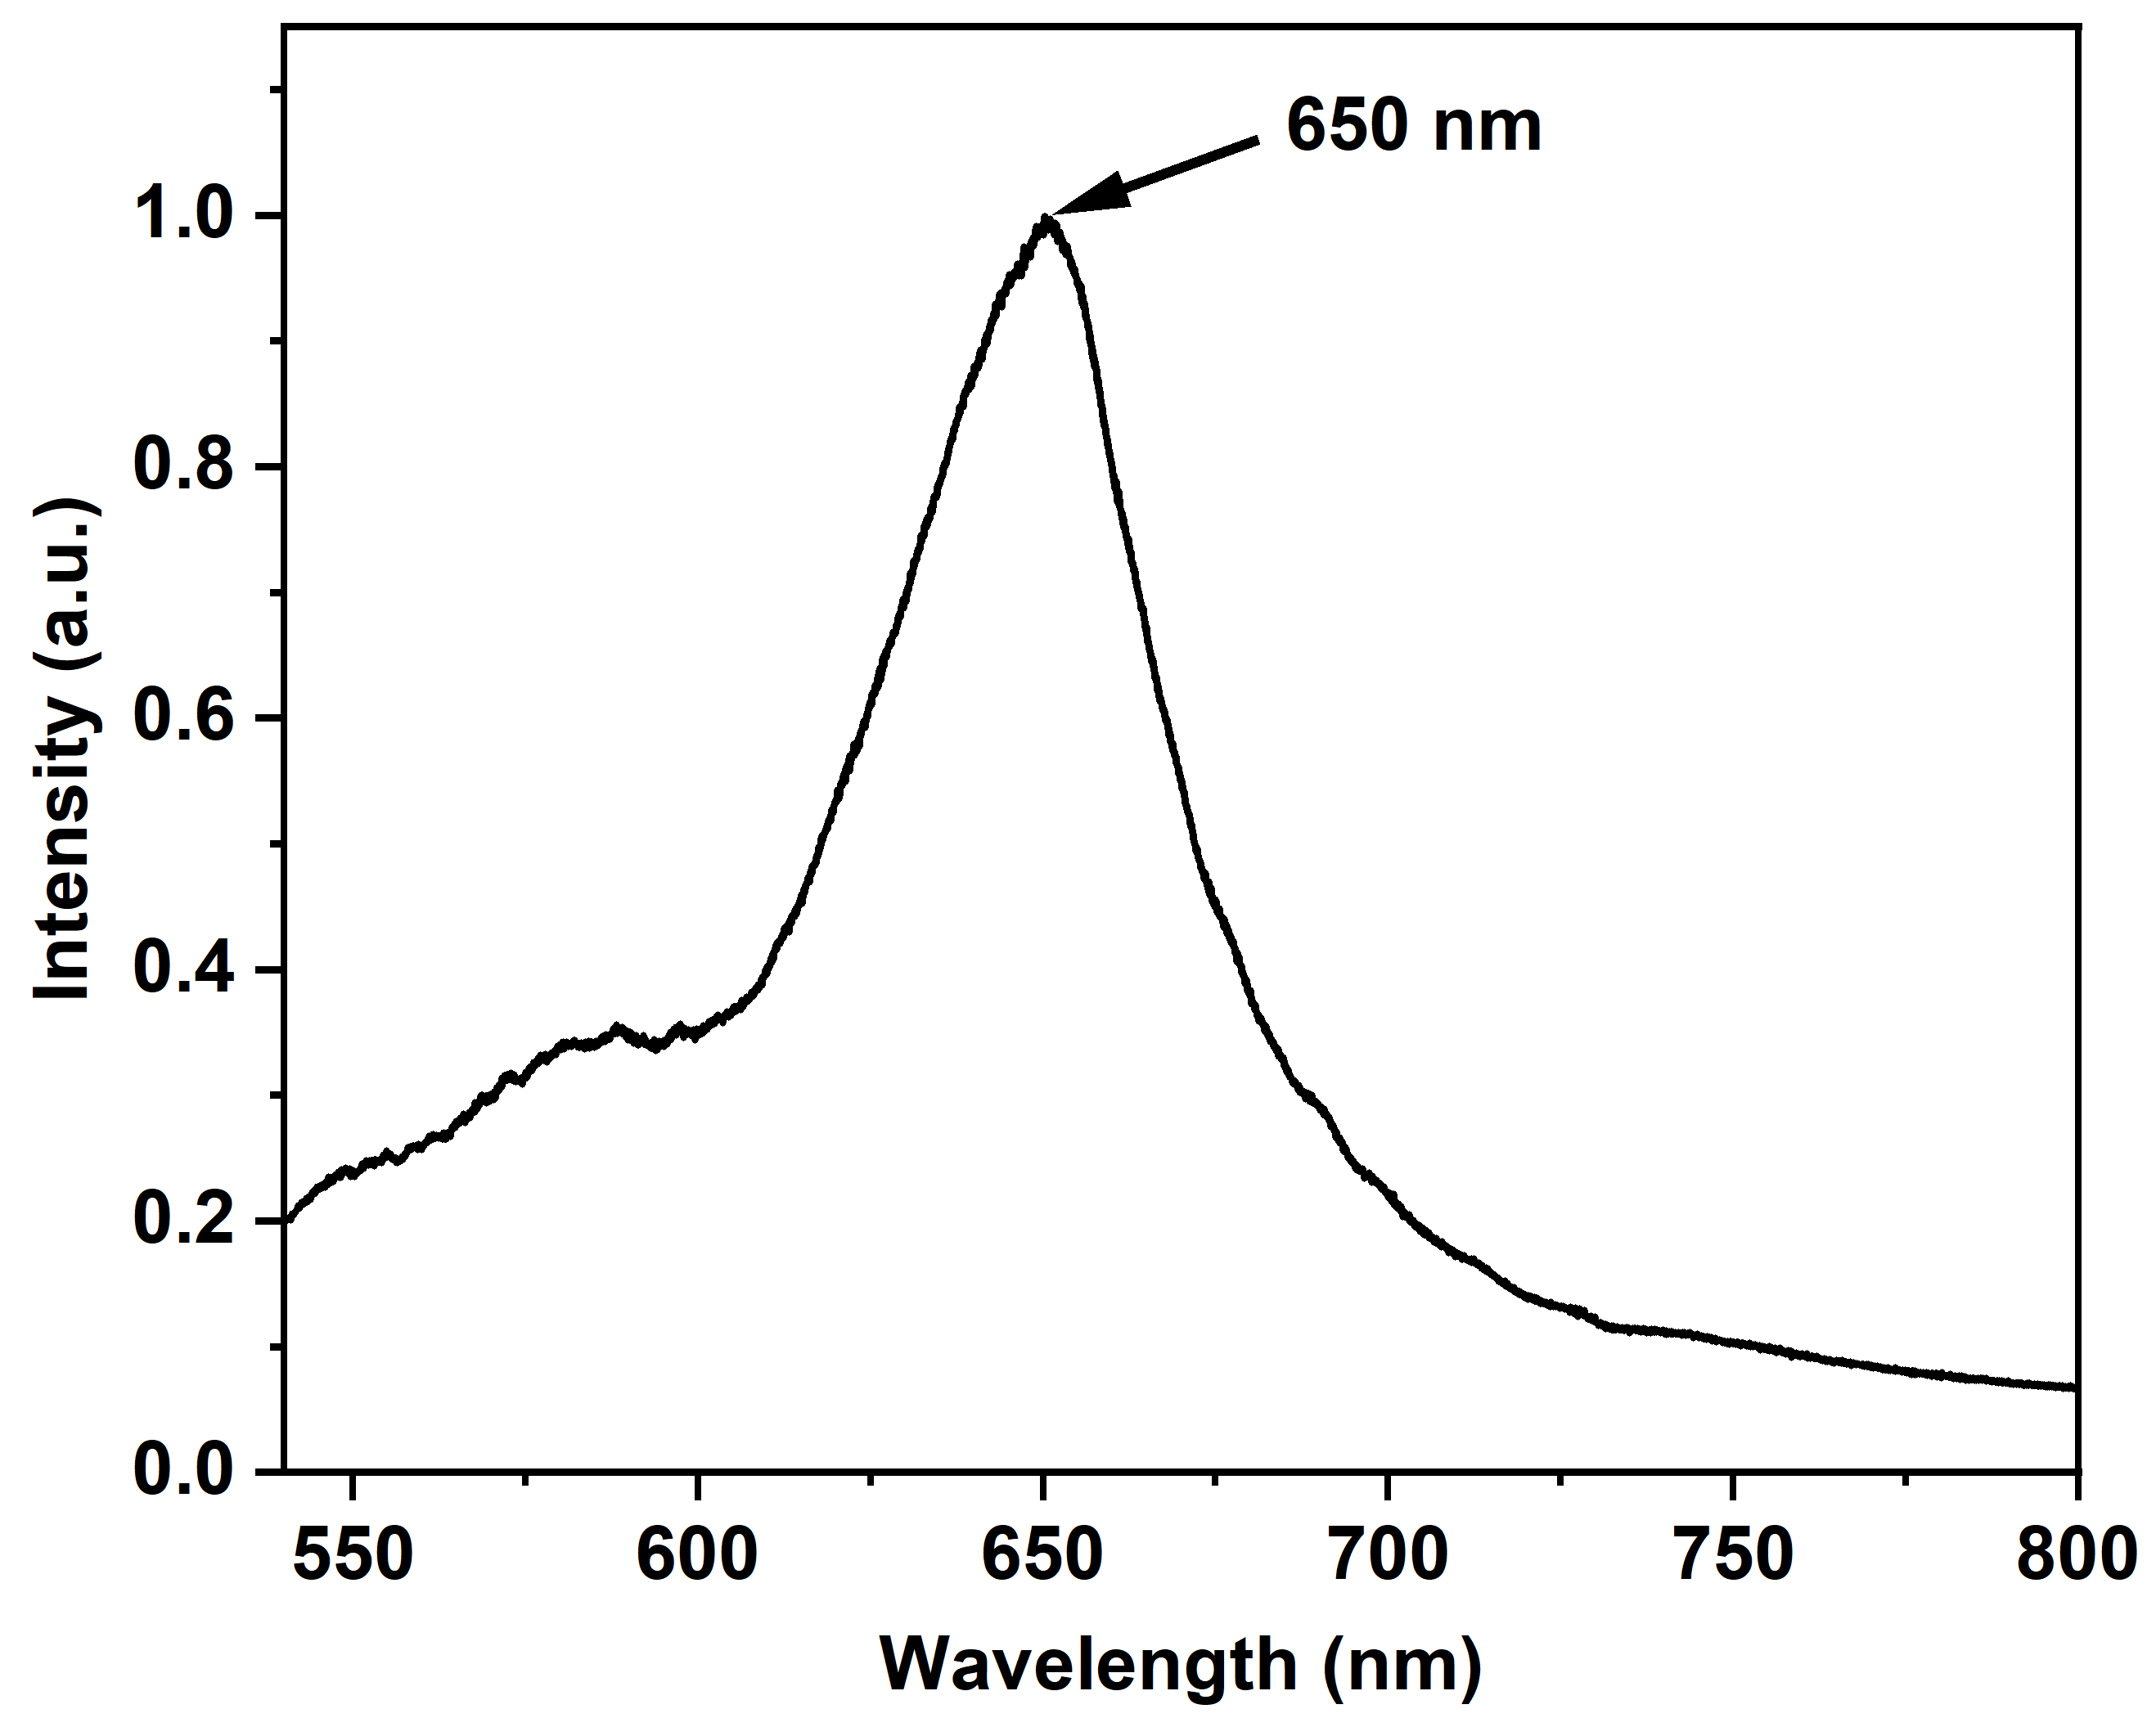
\includegraphics[width=0.75\linewidth]{PL spectra for CdSe_1.png}}
    \caption{\textbf{(a)} Absorption spectrum of CdSe quantum dots with the corresponding Tauc plot shown in the inset. \textbf{(b)} Photoluminescence spectrum of CdSe QDs excited using \textit{532 nm} light.}
    \label{fig:optical spectra}
\end{figure}

Figure \ref{fig:optical spectra} (b) shows the photoluminescence spectrum of CdSe QDs obtained using Horiba LabRAM HR Evolution spectrometer. CdSe QDs solution is excited with a light of 532 nm wavelength. The peak observed at 650 nm is assumed to originate from band-edge emission since it shows red-shift with increase in temperature (not shown in the figure). The defect state emissions in this CdSe QDs solution are very weak and not seen in the photoluminescence spectrum. Hence the photoluminescence emission is strongly a function of the size of CdSe QDs. Due to the presence of QDs of different sizes in the solution, and each QD contributes to the emission at different frequencies, the resulting spectrum is inhomogeneously broadened. Hence, it results in an origin of lifetime distribution as shown in Figure \ref{fig:lifetime histogram}.


\bibliography{aipsamp}

\end{document}
%
% ****** End of file aipsamp.tex ******